\PassOptionsToPackage{dvipsnames}{xcolor}

\documentclass[10pt]{article} % For LaTeX2e
\usepackage[preprint]{tmlr}
% If accepted, instead use the following line for the camera-ready submission:
%\usepackage[accepted]{tmlr}
% To de-anonymize and remove mentions to TMLR (for example for posting to preprint servers), instead use the following:
%\usepackage[preprint]{tmlr}

\usepackage{amssymb,amsmath,amsthm,mathtools}
\usepackage{hyperref}
\usepackage{url}
\usepackage{upquote}
\usepackage{booktabs}

\usepackage{microtype}
\UseMicrotypeSet[protrusion]{basicmath} % disable protrusion for tt fonts

\usepackage{xcolor}

\usepackage{hyperref}
\hypersetup{
  colorlinks = true,
  breaklinks = true,
  linkcolor  = black,
  filecolor  = MidnightBlue,
  citecolor  = MidnightBlue,
  urlcolor   = MidnightBlue
}

\usepackage{cleveref}

% Optional math commands from https://github.com/goodfeli/dlbook_notation.
%%%%% NEW MATH DEFINITIONS %%%%%

% Mark sections of captions for referring to divisions of figures
\newcommand{\figleft}{{\em (Left)}}
\newcommand{\figcenter}{{\em (Center)}}
\newcommand{\figright}{{\em (Right)}}
\newcommand{\figtop}{{\em (Top)}}
\newcommand{\figbottom}{{\em (Bottom)}}
\newcommand{\captiona}{{\em (a)}}
\newcommand{\captionb}{{\em (b)}}
\newcommand{\captionc}{{\em (c)}}
\newcommand{\captiond}{{\em (d)}}

% Highlight a newly defined term
\newcommand{\newterm}[1]{{\bf #1}}

% Figure reference, lower-case.
\def\figref#1{figure~\ref{#1}}
% Figure reference, capital. For start of sentence
\def\Figref#1{Figure~\ref{#1}}
\def\twofigref#1#2{figures \ref{#1} and \ref{#2}}
\def\quadfigref#1#2#3#4{figures \ref{#1}, \ref{#2}, \ref{#3} and \ref{#4}}
% Section reference, lower-case.
\def\secref#1{section~\ref{#1}}
% Section reference, capital.
\def\Secref#1{Section~\ref{#1}}
% Reference to two sections.
\def\twosecrefs#1#2{sections \ref{#1} and \ref{#2}}
% Reference to three sections.
\def\secrefs#1#2#3{sections \ref{#1}, \ref{#2} and \ref{#3}}
% Reference to an equation, lower-case.
\def\eqref#1{equation~\ref{#1}}
% Reference to an equation, upper case
\def\Eqref#1{Equation~\ref{#1}}
% A raw reference to an equation---avoid using if possible
\def\plaineqref#1{\ref{#1}}
% Reference to a chapter, lower-case.
\def\chapref#1{chapter~\ref{#1}}
% Reference to an equation, upper case.
\def\Chapref#1{Chapter~\ref{#1}}
% Reference to a range of chapters
\def\rangechapref#1#2{chapters\ref{#1}--\ref{#2}}
% Reference to an algorithm, lower-case.
\def\algref#1{algorithm~\ref{#1}}
% Reference to an algorithm, upper case.
\def\Algref#1{Algorithm~\ref{#1}}
\def\twoalgref#1#2{algorithms \ref{#1} and \ref{#2}}
\def\Twoalgref#1#2{Algorithms \ref{#1} and \ref{#2}}
% Reference to a part, lower case
\def\partref#1{part~\ref{#1}}
% Reference to a part, upper case
\def\Partref#1{Part~\ref{#1}}
\def\twopartref#1#2{parts \ref{#1} and \ref{#2}}

\def\ceil#1{\lceil #1 \rceil}
\def\floor#1{\lfloor #1 \rfloor}
\def\1{\bm{1}}
\newcommand{\train}{\mathcal{D}}
\newcommand{\valid}{\mathcal{D_{\mathrm{valid}}}}
\newcommand{\test}{\mathcal{D_{\mathrm{test}}}}

\def\eps{{\epsilon}}

% Random variables
\def\reta{{\textnormal{$\eta$}}}
\def\ra{{\textnormal{a}}}
\def\rb{{\textnormal{b}}}
\def\rc{{\textnormal{c}}}
\def\rd{{\textnormal{d}}}
\def\re{{\textnormal{e}}}
\def\rf{{\textnormal{f}}}
\def\rg{{\textnormal{g}}}
\def\rh{{\textnormal{h}}}
\def\ri{{\textnormal{i}}}
\def\rj{{\textnormal{j}}}
\def\rk{{\textnormal{k}}}
\def\rl{{\textnormal{l}}}
% rm is already a command, just don't name any random variables m
\def\rn{{\textnormal{n}}}
\def\ro{{\textnormal{o}}}
\def\rp{{\textnormal{p}}}
\def\rq{{\textnormal{q}}}
\def\rr{{\textnormal{r}}}
\def\rs{{\textnormal{s}}}
\def\rt{{\textnormal{t}}}
\def\ru{{\textnormal{u}}}
\def\rv{{\textnormal{v}}}
\def\rw{{\textnormal{w}}}
\def\rx{{\textnormal{x}}}
\def\ry{{\textnormal{y}}}
\def\rz{{\textnormal{z}}}

% Random vectors
\def\rvepsilon{{\mathbf{\epsilon}}}
\def\rvtheta{{\mathbf{\theta}}}
\def\rva{{\mathbf{a}}}
\def\rvb{{\mathbf{b}}}
\def\rvc{{\mathbf{c}}}
\def\rvd{{\mathbf{d}}}
\def\rve{{\mathbf{e}}}
\def\rvf{{\mathbf{f}}}
\def\rvg{{\mathbf{g}}}
\def\rvh{{\mathbf{h}}}
\def\rvu{{\mathbf{i}}}
\def\rvj{{\mathbf{j}}}
\def\rvk{{\mathbf{k}}}
\def\rvl{{\mathbf{l}}}
\def\rvm{{\mathbf{m}}}
\def\rvn{{\mathbf{n}}}
\def\rvo{{\mathbf{o}}}
\def\rvp{{\mathbf{p}}}
\def\rvq{{\mathbf{q}}}
\def\rvr{{\mathbf{r}}}
\def\rvs{{\mathbf{s}}}
\def\rvt{{\mathbf{t}}}
\def\rvu{{\mathbf{u}}}
\def\rvv{{\mathbf{v}}}
\def\rvw{{\mathbf{w}}}
\def\rvx{{\mathbf{x}}}
\def\rvy{{\mathbf{y}}}
\def\rvz{{\mathbf{z}}}

% Elements of random vectors
\def\erva{{\textnormal{a}}}
\def\ervb{{\textnormal{b}}}
\def\ervc{{\textnormal{c}}}
\def\ervd{{\textnormal{d}}}
\def\erve{{\textnormal{e}}}
\def\ervf{{\textnormal{f}}}
\def\ervg{{\textnormal{g}}}
\def\ervh{{\textnormal{h}}}
\def\ervi{{\textnormal{i}}}
\def\ervj{{\textnormal{j}}}
\def\ervk{{\textnormal{k}}}
\def\ervl{{\textnormal{l}}}
\def\ervm{{\textnormal{m}}}
\def\ervn{{\textnormal{n}}}
\def\ervo{{\textnormal{o}}}
\def\ervp{{\textnormal{p}}}
\def\ervq{{\textnormal{q}}}
\def\ervr{{\textnormal{r}}}
\def\ervs{{\textnormal{s}}}
\def\ervt{{\textnormal{t}}}
\def\ervu{{\textnormal{u}}}
\def\ervv{{\textnormal{v}}}
\def\ervw{{\textnormal{w}}}
\def\ervx{{\textnormal{x}}}
\def\ervy{{\textnormal{y}}}
\def\ervz{{\textnormal{z}}}

% Random matrices
\def\rmA{{\mathbf{A}}}
\def\rmB{{\mathbf{B}}}
\def\rmC{{\mathbf{C}}}
\def\rmD{{\mathbf{D}}}
\def\rmE{{\mathbf{E}}}
\def\rmF{{\mathbf{F}}}
\def\rmG{{\mathbf{G}}}
\def\rmH{{\mathbf{H}}}
\def\rmI{{\mathbf{I}}}
\def\rmJ{{\mathbf{J}}}
\def\rmK{{\mathbf{K}}}
\def\rmL{{\mathbf{L}}}
\def\rmM{{\mathbf{M}}}
\def\rmN{{\mathbf{N}}}
\def\rmO{{\mathbf{O}}}
\def\rmP{{\mathbf{P}}}
\def\rmQ{{\mathbf{Q}}}
\def\rmR{{\mathbf{R}}}
\def\rmS{{\mathbf{S}}}
\def\rmT{{\mathbf{T}}}
\def\rmU{{\mathbf{U}}}
\def\rmV{{\mathbf{V}}}
\def\rmW{{\mathbf{W}}}
\def\rmX{{\mathbf{X}}}
\def\rmY{{\mathbf{Y}}}
\def\rmZ{{\mathbf{Z}}}

% Elements of random matrices
\def\ermA{{\textnormal{A}}}
\def\ermB{{\textnormal{B}}}
\def\ermC{{\textnormal{C}}}
\def\ermD{{\textnormal{D}}}
\def\ermE{{\textnormal{E}}}
\def\ermF{{\textnormal{F}}}
\def\ermG{{\textnormal{G}}}
\def\ermH{{\textnormal{H}}}
\def\ermI{{\textnormal{I}}}
\def\ermJ{{\textnormal{J}}}
\def\ermK{{\textnormal{K}}}
\def\ermL{{\textnormal{L}}}
\def\ermM{{\textnormal{M}}}
\def\ermN{{\textnormal{N}}}
\def\ermO{{\textnormal{O}}}
\def\ermP{{\textnormal{P}}}
\def\ermQ{{\textnormal{Q}}}
\def\ermR{{\textnormal{R}}}
\def\ermS{{\textnormal{S}}}
\def\ermT{{\textnormal{T}}}
\def\ermU{{\textnormal{U}}}
\def\ermV{{\textnormal{V}}}
\def\ermW{{\textnormal{W}}}
\def\ermX{{\textnormal{X}}}
\def\ermY{{\textnormal{Y}}}
\def\ermZ{{\textnormal{Z}}}

% Vectors
\def\vzero{{\bm{0}}}
\def\vone{{\bm{1}}}
\def\vmu{{\bm{\mu}}}
\def\vtheta{{\bm{\theta}}}
\def\va{{\bm{a}}}
\def\vb{{\bm{b}}}
\def\vc{{\bm{c}}}
\def\vd{{\bm{d}}}
\def\ve{{\bm{e}}}
\def\vf{{\bm{f}}}
\def\vg{{\bm{g}}}
\def\vh{{\bm{h}}}
\def\vi{{\bm{i}}}
\def\vj{{\bm{j}}}
\def\vk{{\bm{k}}}
\def\vl{{\bm{l}}}
\def\vm{{\bm{m}}}
\def\vn{{\bm{n}}}
\def\vo{{\bm{o}}}
\def\vp{{\bm{p}}}
\def\vq{{\bm{q}}}
\def\vr{{\bm{r}}}
\def\vs{{\bm{s}}}
\def\vt{{\bm{t}}}
\def\vu{{\bm{u}}}
\def\vv{{\bm{v}}}
\def\vw{{\bm{w}}}
\def\vx{{\bm{x}}}
\def\vy{{\bm{y}}}
\def\vz{{\bm{z}}}

% Elements of vectors
\def\evalpha{{\alpha}}
\def\evbeta{{\beta}}
\def\evepsilon{{\epsilon}}
\def\evlambda{{\lambda}}
\def\evomega{{\omega}}
\def\evmu{{\mu}}
\def\evpsi{{\psi}}
\def\evsigma{{\sigma}}
\def\evtheta{{\theta}}
\def\eva{{a}}
\def\evb{{b}}
\def\evc{{c}}
\def\evd{{d}}
\def\eve{{e}}
\def\evf{{f}}
\def\evg{{g}}
\def\evh{{h}}
\def\evi{{i}}
\def\evj{{j}}
\def\evk{{k}}
\def\evl{{l}}
\def\evm{{m}}
\def\evn{{n}}
\def\evo{{o}}
\def\evp{{p}}
\def\evq{{q}}
\def\evr{{r}}
\def\evs{{s}}
\def\evt{{t}}
\def\evu{{u}}
\def\evv{{v}}
\def\evw{{w}}
\def\evx{{x}}
\def\evy{{y}}
\def\evz{{z}}

% Matrix
\def\mA{{\bm{A}}}
\def\mB{{\bm{B}}}
\def\mC{{\bm{C}}}
\def\mD{{\bm{D}}}
\def\mE{{\bm{E}}}
\def\mF{{\bm{F}}}
\def\mG{{\bm{G}}}
\def\mH{{\bm{H}}}
\def\mI{{\bm{I}}}
\def\mJ{{\bm{J}}}
\def\mK{{\bm{K}}}
\def\mL{{\bm{L}}}
\def\mM{{\bm{M}}}
\def\mN{{\bm{N}}}
\def\mO{{\bm{O}}}
\def\mP{{\bm{P}}}
\def\mQ{{\bm{Q}}}
\def\mR{{\bm{R}}}
\def\mS{{\bm{S}}}
\def\mT{{\bm{T}}}
\def\mU{{\bm{U}}}
\def\mV{{\bm{V}}}
\def\mW{{\bm{W}}}
\def\mX{{\bm{X}}}
\def\mY{{\bm{Y}}}
\def\mZ{{\bm{Z}}}
\def\mBeta{{\bm{\beta}}}
\def\mPhi{{\bm{\Phi}}}
\def\mLambda{{\bm{\Lambda}}}
\def\mSigma{{\bm{\Sigma}}}

% Tensor
\DeclareMathAlphabet{\mathsfit}{\encodingdefault}{\sfdefault}{m}{sl}
\SetMathAlphabet{\mathsfit}{bold}{\encodingdefault}{\sfdefault}{bx}{n}
\newcommand{\tens}[1]{\bm{\mathsfit{#1}}}
\def\tA{{\tens{A}}}
\def\tB{{\tens{B}}}
\def\tC{{\tens{C}}}
\def\tD{{\tens{D}}}
\def\tE{{\tens{E}}}
\def\tF{{\tens{F}}}
\def\tG{{\tens{G}}}
\def\tH{{\tens{H}}}
\def\tI{{\tens{I}}}
\def\tJ{{\tens{J}}}
\def\tK{{\tens{K}}}
\def\tL{{\tens{L}}}
\def\tM{{\tens{M}}}
\def\tN{{\tens{N}}}
\def\tO{{\tens{O}}}
\def\tP{{\tens{P}}}
\def\tQ{{\tens{Q}}}
\def\tR{{\tens{R}}}
\def\tS{{\tens{S}}}
\def\tT{{\tens{T}}}
\def\tU{{\tens{U}}}
\def\tV{{\tens{V}}}
\def\tW{{\tens{W}}}
\def\tX{{\tens{X}}}
\def\tY{{\tens{Y}}}
\def\tZ{{\tens{Z}}}

% Graph
\def\gA{{\mathcal{A}}}
\def\gB{{\mathcal{B}}}
\def\gC{{\mathcal{C}}}
\def\gD{{\mathcal{D}}}
\def\gE{{\mathcal{E}}}
\def\gF{{\mathcal{F}}}
\def\gG{{\mathcal{G}}}
\def\gH{{\mathcal{H}}}
\def\gI{{\mathcal{I}}}
\def\gJ{{\mathcal{J}}}
\def\gK{{\mathcal{K}}}
\def\gL{{\mathcal{L}}}
\def\gM{{\mathcal{M}}}
\def\gN{{\mathcal{N}}}
\def\gO{{\mathcal{O}}}
\def\gP{{\mathcal{P}}}
\def\gQ{{\mathcal{Q}}}
\def\gR{{\mathcal{R}}}
\def\gS{{\mathcal{S}}}
\def\gT{{\mathcal{T}}}
\def\gU{{\mathcal{U}}}
\def\gV{{\mathcal{V}}}
\def\gW{{\mathcal{W}}}
\def\gX{{\mathcal{X}}}
\def\gY{{\mathcal{Y}}}
\def\gZ{{\mathcal{Z}}}

% Sets
\def\sA{{\mathbb{A}}}
\def\sB{{\mathbb{B}}}
\def\sC{{\mathbb{C}}}
\def\sD{{\mathbb{D}}}
% Don't use a set called E, because this would be the same as our symbol
% for expectation.
\def\sF{{\mathbb{F}}}
\def\sG{{\mathbb{G}}}
\def\sH{{\mathbb{H}}}
\def\sI{{\mathbb{I}}}
\def\sJ{{\mathbb{J}}}
\def\sK{{\mathbb{K}}}
\def\sL{{\mathbb{L}}}
\def\sM{{\mathbb{M}}}
\def\sN{{\mathbb{N}}}
\def\sO{{\mathbb{O}}}
\def\sP{{\mathbb{P}}}
\def\sQ{{\mathbb{Q}}}
\def\sR{{\mathbb{R}}}
\def\sS{{\mathbb{S}}}
\def\sT{{\mathbb{T}}}
\def\sU{{\mathbb{U}}}
\def\sV{{\mathbb{V}}}
\def\sW{{\mathbb{W}}}
\def\sX{{\mathbb{X}}}
\def\sY{{\mathbb{Y}}}
\def\sZ{{\mathbb{Z}}}

% Entries of a matrix
\def\emLambda{{\Lambda}}
\def\emA{{A}}
\def\emB{{B}}
\def\emC{{C}}
\def\emD{{D}}
\def\emE{{E}}
\def\emF{{F}}
\def\emG{{G}}
\def\emH{{H}}
\def\emI{{I}}
\def\emJ{{J}}
\def\emK{{K}}
\def\emL{{L}}
\def\emM{{M}}
\def\emN{{N}}
\def\emO{{O}}
\def\emP{{P}}
\def\emQ{{Q}}
\def\emR{{R}}
\def\emS{{S}}
\def\emT{{T}}
\def\emU{{U}}
\def\emV{{V}}
\def\emW{{W}}
\def\emX{{X}}
\def\emY{{Y}}
\def\emZ{{Z}}
\def\emSigma{{\Sigma}}

% entries of a tensor
% Same font as tensor, without \bm wrapper
\newcommand{\etens}[1]{\mathsfit{#1}}
\def\etLambda{{\etens{\Lambda}}}
\def\etA{{\etens{A}}}
\def\etB{{\etens{B}}}
\def\etC{{\etens{C}}}
\def\etD{{\etens{D}}}
\def\etE{{\etens{E}}}
\def\etF{{\etens{F}}}
\def\etG{{\etens{G}}}
\def\etH{{\etens{H}}}
\def\etI{{\etens{I}}}
\def\etJ{{\etens{J}}}
\def\etK{{\etens{K}}}
\def\etL{{\etens{L}}}
\def\etM{{\etens{M}}}
\def\etN{{\etens{N}}}
\def\etO{{\etens{O}}}
\def\etP{{\etens{P}}}
\def\etQ{{\etens{Q}}}
\def\etR{{\etens{R}}}
\def\etS{{\etens{S}}}
\def\etT{{\etens{T}}}
\def\etU{{\etens{U}}}
\def\etV{{\etens{V}}}
\def\etW{{\etens{W}}}
\def\etX{{\etens{X}}}
\def\etY{{\etens{Y}}}
\def\etZ{{\etens{Z}}}

% The true underlying data generating distribution
\newcommand{\pdata}{p_{\rm{data}}}
% The empirical distribution defined by the training set
\newcommand{\ptrain}{\hat{p}_{\rm{data}}}
\newcommand{\Ptrain}{\hat{P}_{\rm{data}}}
% The model distribution
\newcommand{\pmodel}{p_{\rm{model}}}
\newcommand{\Pmodel}{P_{\rm{model}}}
\newcommand{\ptildemodel}{\tilde{p}_{\rm{model}}}
% Stochastic autoencoder distributions
\newcommand{\pencode}{p_{\rm{encoder}}}
\newcommand{\pdecode}{p_{\rm{decoder}}}
\newcommand{\precons}{p_{\rm{reconstruct}}}

\newcommand{\laplace}{\mathrm{Laplace}} % Laplace distribution

% \newcommand{\E}{\mathbb{E}}
\newcommand{\Ls}{\mathcal{L}}
\newcommand{\R}{\mathbb{R}}
\newcommand{\emp}{\tilde{p}}
\newcommand{\lr}{\alpha}
\newcommand{\reg}{\lambda}
\newcommand{\rect}{\mathrm{rectifier}}
\newcommand{\softmax}{\mathrm{softmax}}
\newcommand{\sigmoid}{\sigma}
\newcommand{\softplus}{\zeta}
\newcommand{\KL}{D_{\mathrm{KL}}}
\newcommand{\Var}{\mathrm{Var}}
\newcommand{\standarderror}{\mathrm{SE}}
\newcommand{\Cov}{\mathrm{Cov}}
% Wolfram Mathworld says $L^2$ is for function spaces and $\ell^2$ is for vectors
% But then they seem to use $L^2$ for vectors throughout the site, and so does
% wikipedia.
\newcommand{\normlzero}{L^0}
\newcommand{\normlone}{L^1}
\newcommand{\normltwo}{L^2}
\newcommand{\normlp}{L^p}
\newcommand{\normmax}{L^\infty}

\newcommand{\parents}{Pa} % See usage in notation.tex. Chosen to match Daphne's book.

\DeclareMathOperator*{\argmax}{arg\,max}
\DeclareMathOperator*{\argmin}{arg\,min}

\DeclareMathOperator{\sign}{sign}
\DeclareMathOperator{\Tr}{Tr}
\let\ab\allowbreak

% operators
\DeclareMathOperator*{\argmax}{arg\,max}
\DeclareMathOperator*{\argmin}{arg\,min}
\DeclareMathOperator{\E}{E}
\DeclareMathOperator{\var}{Var}
\DeclareMathOperator{\cov}{Cov}
\DeclareMathOperator{\tr}{tr}
\DeclareMathOperator{\diag}{diag}
\DeclareMathOperator{\range}{range}
\DeclareMathOperator{\nullspace}{null}
\DeclareMathOperator{\rank}{rank}
\DeclareMathOperator{\card}{card}
\DeclareMathOperator{\sign}{sign}
\DeclareMathOperator{\st}{S}
\DeclareMathOperator{\normal}{Normal}
\DeclareMathOperator{\fnormal}{FoldedNormal}
\DeclareMathOperator{\bernoulli}{Bernoulli}
\DeclareMathOperator{\erf}{erf}
\DeclareMathOperator{\mse}{MSE}
\DeclareMathOperator{\risk}{R}
% \DeclareMathOperator{\I}{I}
% \DeclareMathOperator{\T}{}
%
% \DeclareMathSymbol{\phi}{\mathalpha}{operators}{0}
\DeclareMathOperator{\pdf}{\phi}
\DeclareMathOperator{\cdf}{\Phi}
% commands
% \newcommand{\vec}{\vectorsym}
% \newcommand{\mat}{\matrixsym}
\renewcommand{\vec}{\boldsymbol}
\newcommand{\mat}{\boldsymbol}
\newcommand*\du{\mathop{}\!\mathrm{d}}
% \newcommand{\T}{\mathsf{T}}
\newcommand{\T}{\intercal}
\newcommand{\ones}{\boldsymbol{1}}
% \newcommand{\T}{\intercal}
% \newcommand{\T}[1]{{1}^{\mathsf{T}}}
\newcommand{\ind}[1]{\operatorname{I}_{#1}}

% environments
\theoremstyle{plain}
\newtheorem{theorem}{Theorem}[section]
\newtheorem{corollary}{Corollary}[theorem]
\newtheorem{lemma}{Lemma}[section]
\newtheorem{proposition}{Proposition}[section]

\theoremstyle{definition}
\newtheorem{definition}{Definition}[section]
\newtheorem{example}{Example}[section]

\theoremstyle{remark}
\newtheorem{remark}[theorem]{Remark}

\newcommand{\todojl}[1]{\todo[color=green!40]{#1}}



\title{Formatting Instructions for TMLR \\Journal Submissions}

% Authors must not appear in the submitted version. They should be hidden
% as long as the tmlr package is used without the [accepted] or [preprint] options.
% Non-anonymous submissions will be rejected without review.

\author{%
  \name Johan Larsson \email johan.larsson@stat.lu.se\\
  \addr Deparment of Statistics\\Lund University
  \AND
  \name Jonas Wallin \email jonas.wallin@stat.lu.se\\
  \addr Department of Statistics\\Lund University
}

% The \author macro works with any number of authors. Use \AND 
% to separate the names and addresses of multiple authors.

\newcommand{\fix}{\marginpar{FIX}}
\newcommand{\new}{\marginpar{NEW}}

\def\month{MM}  % Insert correct month for camera-ready version
\def\year{YYYY} % Insert correct year for camera-ready version
\def\openreview{\url{https://openreview.net/forum?id=XXXX}} % Insert correct link to OpenReview for camera-ready version

\begin{document}

\maketitle

\begin{abstract}
  The abstract paragraph should be indented 1/2~inch on both left and
  right-hand margins. Use 10~point type, with a vertical spacing of 11~points.
  The word \textbf{\large Abstract} must be centered, in bold, and in point size 12. Two
  line spaces precede the abstract. The abstract must be limited to one
  paragraph.
\end{abstract}

\section{Introduction}

When modeling high-dimensional high-dimensional where the number of features \(p\) exceeds
the number of observations \(n\), it is impossible to apply classical statistical models
such as standard linear regression since the design matrix \(\mat X\) is no longer of full
rank. A common remedy to this problem is to \emph{regularize} the model by adding a term to
the objective function that punishes models with large coefficients (\(\vec\beta\)). If we
let \(g(\vec\beta; \mat X, \vec y)\) be the original objective function---which when
minimized improves the model's fit to the data (\(\mat X, \vec y\))---then we are
interested in minimizing the following objective:
\begin{equation}
  \label{eq:general-objective}
  f(\beta_0, \vec\beta; \mat X, \vec y) = g(\beta_0, \vec\beta; \mat X, \vec y) + h(\vec\beta),
\end{equation}
which is composed of \(g\) and a penalty term \(h(\vec\beta)\) that depends only on \(\bm{\beta}\).
Some of the most common penalties are the \(\ell_1\) norm (\(\lVert \vec\beta \rVert_1\)) and squared \(\ell_2\) norm
penalties (\(\lVert \bm{\beta} \rVert_2^2\)), which if \(g\) is the standard ordinary least-squares objective, represent
the lasso~\citep{tibshirani1996,santosa1986,donoho1994} and ridge (Tikhonov) regression
% TODO: insert reference for ridge regression
respectively. Other common penalties include the sorted \(\ell_1\)-norm used in Sorted
L-One Penalized Estimation (SLOPE)~\citep{bogdan2013,zeng2014,bogdan2015}, the
minimax-concave penalty (MCP)~\citep{zhang2010}, hinge loss (used in support vector
machines~\citep{cortes1995}) and smoothly-clipped absolute
deviation~(SCAD)~\citep{fan2001}. Many penalities---indeed all of the mentioned
ones---shrink coefficients in proportion to their sizes.

The issue with this type of shrinkage is that it is sensitive to the scales of the features
in \(\mat X\). To avoid this it is common to \emph{normalize} the features before fitting
the model by shifting and scaling each feature by measures of location and scale
respectively. For some problems such measures arise naturally from contextual knowledge
about the problem, but in most cases they must be estimated from data. A popular strategy
is to use the mean and standard deviation of each feature as location and scale factors
respectively, which is called \emph{standardization}. Most types of normalization are based
only on the marginal distributions of the features, but there are exceptions such as the
adaptive lasso~\citep{zou2006}. Another reason for normalizing the features is to improve
properties of optimization algorithms used to fit the model, but we will not consider this
topic here.

The choice of normalization may have consequences for the estimated model. As a first
example of this, consider \Cref{fig:realdata-paths}, which displays the lasso paths for
four real data sets and two different types of normalization. For most of the datasets, the
models differ significantly depending on type of normalization, yielding differences in
terms of feature selection as well as signs and magnitudes of the corresponding
coefficients.

% TODO: reduce image to one row?
\begin{figure}[bpt]
  \centering
  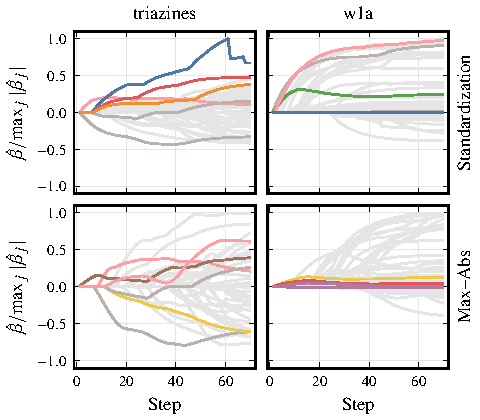
\includegraphics[]{plots/realdata_paths_small.pdf}
  \caption{%
    Lasso paths for real datasets using two types of normalization:
    standardization and maximum absolute value normalization (max--abs). We have fit
    the lasso path to two different datasets:
    \data{triazines}~\citep{king} and \data{w1a}~\citep{platt1998}. (See \Cref{sec:data-summary}
    for more information about these data sets.) For each
    dataset, we have colored the coefficients if they were among the first five
    to become non-zero under either of the two normalization schemes.
  }
  \label{fig:realdata-paths}
\end{figure}

In spite of this relationship between normalization and regularization, there has so far
been no research on the topic. Instead, the choice of normalization is often motivated by
being standard. And sometimes the choice is based on computational aspects such as
optimization performance and data storage. At the time of writing, for instance, the
popular machine learning library \texttt{scikit-learn}~\citep{scikit-learndevelopers2024}
recommends maximum absolute value normalization in the particular case of sparse data. Yet,
as we have already seen (\Cref{fig:realdata-paths}), this may have dramatic effects for the
results.

Standardization is a natural choice when the features are normally distributed. But for
other types of data the choice is not as straightforward. There is for instance no clear
approach to normalizing binary features (where the each observations takes either of only
two values). Anecdotal suggestions include not normalizing at all or to normalize as you
would if it were continuous data---the implications of either of these suggestions (or in
deed any other), however, have yet to be investigated.

In this paper we will begin to bridge this knowledge gap by studying normalization in the
context of binary data. We will focus on three models that each correspond to a particular
case of \Cref{eq:general-objective}: the lasso, ridge, and elastic net~\citep{zou2005}. The
latter of these, the elastic net, is a generalization of the previous two, and is
represented by the following optimization problem:
%
\begin{multline}
  \label{eq:elastic-net}
  \operatorname*{minimize}_{\beta_0 \in \mathbb{R},\vec{\beta} \in \mathbb{R}^p}\bigg( f(\beta_0, \vec{\beta};\vec{X},\vec{y},\lambda_1,\lambda_2)= \\
  \frac{1}{2} \lVert \vec y - \beta_0 - \tilde{\mat{X}}\vec{\beta} \rVert^2_2  + \lambda_1 \lVert \vec\beta \rVert_1 + \frac{\lambda_2}{2}\lVert \vec \beta \rVert_2^2\bigg).
\end{multline}
%
Setting \(\lambda_1 = 0\) results in the ridge regression objective, whereas \(\lambda_2 =
0\) gives us the lasso. These methods are staples in the field of statistics and machine
learning and are accompanied by a large body of theoretical work and applications for real
data.

We pay particular attention to the case when binary features are imbalanced, that is, have
relatively many ones or zeroes. In this scenario, we demonstrate that the choice of
normalization directly influences the estimated regression coefficients and that this
effect is different for the lasso and ridge regression. In the case of the lasso, we show
that this bias can be mitigated by scaling with variance but that this comes at the cost of
increased variance. For ridge regression we show that scaling by standard deviation
achieves the same effect. In the case of the elastic net, however, we show that there is no
simple normalization method that can mitigate this bias but that it is possible to
circumvent it by instead weighting the penalty terms in the elastic net.

We also study the case of mixed data and show that the choice of normalization has implicit
consequences for the relative weighting of binary and normal features, even in the case
when the binary features are balanced. If we believe, for instance, that a unit change in
the binary variable should equal a certain change in the normal variable (say, two standard
deviations), then scaling must be modified to take this into account.

% TODO: complete this paragraph
Finally, we look at a simple case of interactions between normal and binary features, and
demonstrate what?


\section{Preliminaries}

Throughout this paper, we assume that the data is generated from a linear model, \(y_i =
\beta_0^* + \vec x_i^\T \vec\beta^* + \varepsilon_i\) for \(i \in [n]\) where \([n] =
\{1,2,\dots,n\}\) and we use \(\beta_0^*\) and \(\vec\beta^*\) to denote the true intercept
and coefficients, respectively, and \(\varepsilon_i\) to denote measurement noise. \(\mat
X\) is the \(n \times p\) design matrix with features \(\vec x_j\) and \(\vec y\) the \(n
\times 1\) response vector. Furthermore, we use \(\hat\beta_0\) and \(\hat{\vec{\beta}}\)
to denote our estimates of the intercept and coefficients. We will also assume \(\mat{X}\),
\(\beta_0^*\), and \(\vec{\beta}^*\) to be fixed.

There is considerable ambiguity regarding key terms in the literature. Here, we define
\emph{normalization} as the process of centering and scaling the feature matrix, which we
now formalize.

\begin{definition}[Normalization]
  \label{def:normalization}
  Let \(\tilde{\mat X}\) be the normalized feature matrix with elements
  \(\tilde{x}_{ij} = (x_{ij} - c_{j})/s_j\), where \(x_{ij}\) is an element of
  \(\mat{X}\) and \(c_j\) and \(s_j\) are the \emph{centering} and
  \emph{scaling} factors respectively.
\end{definition}

% Some authors refer to the procedure in \Cref{def:normalization} as \emph{standardization},
% but here we define standardization only as the case when centering with the mean and
% scaling with the (uncorrected) standard deviation.

\subsection{Types of Normalization}

There are many different strategies for normalizing the design matrix. We list a few common
choices in \Cref{tab:normalization-types}. Standardization is perhaps the most popular type
of normalization, at least in the field of statistics. One of its benefits is that it
simplifies certain aspects of fitting the model, such as fitting the intercept. The
downside of standardization is that it involves centering by the mean, which destroys
sparsity. This is not a problem when \(\bm{X}\) is stored as a dense matrix; but when the
data is sparse, it may increase memory use and processing time.

% TODO: move to appendix?
\begin{table}[hbt]
  \centering
  \caption{
    Common ways to normalize a matrix of features using centering and scaling
    factors \(c_j\) and \(s_j\), respectively. Note that \(\bar{x}_j =
    n^{-1}\sum_{i=1}^n x_{ij}\).
  }
  \label{tab:normalization-types}
  \vskip 0.15in
  \small
  \begin{tabular}{lll}
    \toprule
    Normalization            & \(c_{j}\)          & \(s_j\)                                                   \\
    \midrule
    Standardization          & \(\bar{x}_j\)      & \(\sqrt{\frac{1}{n}\sum_{i=1}^n (x_{ij} - \bar{x}_j)^2}\) \\
    \addlinespace
    Max--Abs                 & 0                  & \(\max_i|x_{ij}|\)                                        \\
    \addlinespace
    Min--Max                 & \(\min_i(x_{ij})\) & \(\max_i(x_{ij}) - \min_i(x_{ij})\)                       \\
    \addlinespace
    \(\ell_1\)-Normalization & 0 or \(\bar{x}_j\) & \(\lVert \vec{x}_j\rVert_1\)                              \\
    \addlinespace
    Adaptive Lasso           & 0                  & \(\hat{\beta}_j^\text{OLS}\)                              \\
    \bottomrule
  \end{tabular}
\end{table}

When the data is sparse, a common alternative to standardization is to scale features by
their maximum absolute values (max--abs normalization). This method has no impact on binary
data\footnote{Except in the extreme case when all values are 0.} and therefore retains
sparsity. For other types of data, it scales the features to take values in the range
\([-1, 1]\). Since the scaling is determined by a single value for each feature, the method
is naturally sensitive to outliers. For many types of data, such as normally distributed
data, it is also often the case that the sample maximum depends on sample size, which often
makes use of the method problematic~(\Cref{thm:maxabs-gev}~(\Cref{sec:additional-theory})).

% TODO: should we study l1-normalization more?
Min-max normalization scales the data to lie in \([0, 1]\). As with the max--abs method,
min-max normalization retains sparsity and also shares its sensitivity to outliers and
sample size. Unlike max--abs scaling, however, min--max scaling is not sensitive to the
\emph{location} of the data, only its \emph{spread}. In \(\ell_1\)-normalization, each
feature is scaled with its sum of absolute value. The method is common in signal
processing. A special case of normalization is the adaptive lasso~\citep{zou2006}, which is
a two-step procedure. First we fit a model such as ordinary least-squares (OLS) or ridge
regression. Then we use the estimated coefficients to scale the features and refit.

\subsection{Lasso, Ridge, and Elastic Net Regression}%
\label{sec:elastic-net-solution}

If we include an intercept and assume that the features of the normalized design matrix are
orthogonal, that is, \(\tilde{\mat{X}}^\intercal \tilde{\mat{X}} =
\diag\left(\tilde{\vec{x}}_1^\T \tilde{\vec{x}}_1, \dots, \tilde{\vec{x}}_p^\intercal
\tilde{\vec{x}}_p\right) \), the solution to the coefficients in the elastic net problem is
given by
%
\begin{equation}
  \label{eq:orthogonal-solution-normalized}
  \hat{\beta}^{(n)}_j = \frac{\st_{\lambda_1}\left(\tilde{\vec{x}}_j^\T \vec{y}\right)}{\tilde{\vec{x}}_j^\T \tilde{\vec{x}}_j + \lambda_2},
  \qquad
  \hat{\beta}_0^{(n)} = \frac{\vec{y}^\T \ones}{n},
\end{equation}
%
where \(\st_\lambda(z) = \sign(z) \max(|z| - \lambda, 0)\) is the soft-thresholding
operator. (See \Cref{sec:elastic-net-estimator} for a derivation of this.)

Normalization changes the optimization problem and its solution, the coefficients, which
will now be on the scale of the normalized features. But we are interested in
\(\hat{\vec{\beta}}\): the coefficients on the scale of the original problem. To obtain
these, we transform the coefficients from the normalized poblem, \(\hat\beta^{(n)}_j\),
back via \(\hat\beta_j = \hat\beta^{(n)}_j/s_j\) for \(j \in [p]\). There is a similar
transformation for the intercept but we omit here since we are not interested in it.

\section{Bias-Variance Tradeoffs in Data with Binary Features}

Now, assume that \(\mat{X}\) and \(\vec{\beta}\) are fixed and that \(\vec{y} = \mat{X}\vec{\beta} + \vec{\varepsilon}\), where \(\varepsilon_i\) is identically and independently distributed noise with mean zero and finite variance \(\sigma_\varepsilon^2\). We are interested in the expected value of \Cref{eq:orthogonal-solution}. Let \(Z = \tilde{\vec{x}}_j^\T \vec{y} = \tilde{\vec{x}}_j^\T(\mat{X}\vec{\beta} + \vec{\varepsilon})\) and \(d_j = s_j\left(\tilde{\vec{x}}_j^\T \tilde{\vec{x}}_j + \lambda_2\right)\) so that \(\hat{\beta}_j = \st_{\lambda_1}(Z)/d_j\). We start by focusing on the numerator, since the denominator, \(d_j\), is fixed. First observe that
\[
  \E Z = \mu = \E \left( \tilde{\vec{x}}_j^\T (\vec{x}_j\beta_j + \vec{\varepsilon}) \right)  = \tilde{\vec{x}}_j^\T\vec{x}_j \beta_j.
\]
And for the variance, we have
\[
  \var Z = \sigma^2 = \var\left(\tilde{\vec{x}}_j ^\T \vec{\varepsilon}\right) = \sigma_\varepsilon^2 \lVert \tilde{\vec{x}}_j\rVert_2^2 .
\]

The expected value of the soft-thresholding estimator is
\begin{align}
  \label{eq:st-expected-value}
  \E \st_\lambda(Z) & = \int_{-\infty}^\infty \st_\lambda(z) f_Z(z) \du z                                                   \nonumber \\
                    & = \int_{-\infty}^\infty \ind{|z| > \lambda} (z -\sign(z)\lambda) f_Z(z) \du z                         \nonumber \\
                    & = \int_{-\infty}^{-\lambda}(z + \lambda)f_Z(z) \du z + \int_{\lambda}^\infty (z - \lambda)f_Z(z) \du z.
\end{align}
And then the bias of \(\hat\beta_j\) with respect to the true coefficient \(\beta_j^*\) is
\begin{equation}
  \label{eq:betahat-bias}
  \E \hat\beta_j - \beta_j^* = \frac{1}{d_j}\E \st_\lambda(Z) - \beta^*_j.
\end{equation}

Finally, we note that the variance of the soft-thresholding estimator is
\begin{equation}
  \label{eq:st-variance}
  \var {S_\lambda(Z)} = \int_{-\infty}^{-\lambda}(z + \lambda)^2f_Z(z) \du z + \int_{\lambda}^\infty (z - \lambda)^2 f_Z(z) \du z - \left(\E \st_\lambda(Z)\right)^2
\end{equation}
and that the variance of the elastic net estimator is therefore
\begin{equation}
  \label{eq:betahat-variance}
  \var \hat\beta_j = \frac{1}{d_j^2} \var \st_\lambda(Z).
\end{equation}

% \subsection{Normally Distributed Noise}

Next, we add the additional assumption that \(\vec{\varepsilon}\) is normally distributed. Then
\[
  Z \sim \normal\left(\tilde{\vec{x}}_j^\T\vec{x}_j \beta_j, \sigma_\varepsilon^2 \lVert \tilde{\vec{x}}_j\rVert_2^2 \right).
\]
Let \(\theta = -\mu -\lambda_1 \) and \(\gamma = \mu - \lambda_1\). Then the expected value of soft-thresholding of \(Z\) is
\begin{align}
  \E \st_{\lambda_1}(Z) & = \int_{-\infty}^\frac{\theta}{\sigma} (\sigma u - \theta) \pdf(u) \du u + \int_{-\frac{\gamma}{\sigma}}^\infty (\sigma u + \gamma) \pdf(u) \du u                                               \nonumber                      \\
                        & = -\theta \cdf\left(\frac{\theta}{\sigma}\right) - \sigma \pdf\left(\frac{\theta}{\sigma}\right) + \gamma \cdf\left(\frac{\gamma}{\sigma}\right) + \sigma \pdf\left(\frac{\gamma}{\sigma}\right) \label{eq:mean-centered-eval}
\end{align}
where \(\pdf(u)\) and \(\cdf(u)\) are the probability density and cumulative distribution functions of the standard normal distribution, respectively.

Next, we consider what the variance of the elastic net estimator looks like.
Starting with the first term on the left-hand side of \Cref{eq:st-variance}, we have
\begin{multline}
  \label{eq:mc-var-part1}
  \int_{-\infty}^{-\lambda_1}(z+ \lambda_1)^2 f_Z(z) \du z = \sigma^2 \int_{-\infty}^{\frac{\theta}{\sigma}} y^2 \pdf(y) \du y + 2 \theta \sigma \int_{-\infty}^{\frac{\theta}{\sigma}} y \pdf(y) \du y + \theta^2 \int_{-\infty}^{\frac{\theta}{\sigma}} \pdf(y) \du y \\
  = \frac{\sigma^2}{2} \left( \erf\left(\frac{\theta}{\sigma\sqrt{2}}\right) - \frac{\theta}{\sigma}\sqrt{\frac{2}{\pi}} \exp\left(-\frac{\theta^2}{2\sigma^2}\right) + 1 \right) + 2 \theta \sigma \pdf \left(\frac{\theta}{\sigma}\right) + \theta^2 \cdf\left(\frac{\theta}{\sigma}\right).
\end{multline}
Similar computations for the second term on the left-hand side of \Cref{eq:st-variance} yield
\begin{multline}
  \label{eq:mc-var-part2}
  \int_{\lambda_1}^{\infty}(z - \lambda_1)^2 f_Z(z) \du z \\
  = \frac{\sigma^2}{2} \left( \erf\left(\frac{\gamma}{\sigma\sqrt{2}}\right) - \frac{\gamma}{\sigma}\sqrt{\frac{2}{\pi}} \exp\left(-\frac{\gamma^2}{2\sigma^2}\right) + 1 \right) + 2 \gamma \sigma \pdf \left(\frac{\gamma}{\sigma}\right) + \gamma^2 \cdf\left(\frac{\gamma}{\sigma}\right).
\end{multline}
Plugging \Cref{eq:mean-centered-eval,eq:mc-var-part1,eq:mc-var-part2} into \Cref{eq:betahat-variance} yields the variance of the estimator. Consequently, we can also compute the mean-squared error via the bias-variance decomposition
\begin{equation}
  \label{eq:betahat-mse}
  \mse (\hat\beta_j, \beta^*_j) = \var\hat\beta_j + \left(\E \hat\beta_j - \beta^*_j\right)^2.
\end{equation}

% \subsubsection{Binary Features}

Our results have so far covered the general case where we have made no assumptions on \(\mat{X}\), except for being non-random. But our main focus in this paper
is the case when \(\vec{x_j}\) is a binary feature with class balance \(q\), that is, \(x_{ij} \in \{0, 1\}\) for all \(i\) and \(\sum_{i=1}^n x_{ij} = nq\).
In this case, we observe that
\[
  \begin{aligned}
    \tilde{\vec{x}}_j^\T \tilde{\vec{x}}_j & = \frac{1}{s_j^2}(\vec{x}_j - \ones c_j)^\T (\vec{x}_j - \ones c_j) = \frac{1}{s^2_j}(nq - 2nq^2 + nq^2) = \frac{nq(1-q)}{s^2_j}, \\
    \tilde{\vec{x}}_j^\T \vec{x}_j         & = \frac{1}{s_j}(\vec{x}_j^\T \vec{x}_j - \vec{x}_j^\T \ones c_j) = \frac{nq(1 - q)}{s_j}.
  \end{aligned}
\]
And consequently
\[
  \mu = \frac{\beta^*_j nq(1 - q)}{s_j}, \qquad \sigma^2 = \frac{\sigma_\varepsilon^2nq(1 - q)}{s^2_j}, \qquad d_j = \frac{nq(1 -q)}{s_j}  + \lambda_2 s_j.
\]
We will allow ourselves to abuse notation and overload the definitions of \(\mu\), \(\sigma^2\), and \(d_j\) as functions of \(q\). Then, an expression for the expected value of the elastic net estimate with respect to \(q\) can be obtained by plugging in \(\mu\) and \(\sigma\) into \Cref{eq:mean-centered-eval}.

We are mainly interested in examining the case when \(\vec{x}_j\) is imbalanced and what effect various approaches to normalizing the features
has on the elastic net estimator. In order to study this, we will parameterize the scaling factors \(s_j\) for \(j  \in [p]\) by \(s_j = (q - q^2)^\delta\), \(\delta \geq 0\).
This includes the cases that we are primary interested in, that is,
\begin{itemize}
  \item \(\delta = 0\): no scaling, which includes min--max and max--abs normalization,
  \item \(\delta = 1/2\): standardization, and
  \item \(\delta = 1\): scaling by the variance.
\end{itemize}
Note that the last of these cases does not correspond to a standard type of normalization. But as we will see, it has some interesting properties in the case of binary features.

A natual consequence of the normal distribution of \(Z\) is that the probability of selection in the elastic net problem is given by
\begin{align*}
  \Pr\left(\hat{\beta}_j \neq 0\right) & = \Pr\left(\st_{\lambda_1}(Z) \neq 0\right)                                                                                         \\
                                       & = \Pr\left(Z > \lambda_1\right) + \Pr\left(Z < -\lambda_1\right)                                                                    \\
                                       & = \cdf\left(\frac{\mu - \lambda_1}{\sigma}\right) + \cdf\left(\frac{- \mu -\lambda_1}{\sigma}\right).                               \\
                                       & = \cdf \left( \frac{\beta_j^*n (q-q^2)^{1/2} - \lambda_1(q-q^2)^{\delta - 1/2}}{\sigma_\varepsilon \sqrt{n}}\right)                 \\
                                       & \phantom{={}} + \cdf \left( \frac{-\beta_j^*n (q-q^2)^{1/2} - \lambda_1(q-q^2)^{\delta - 1/2}}{\sigma_\varepsilon \sqrt{n}}\right).
\end{align*}

Letting \(\theta = -\mu - \lambda_1 \) and \(\gamma = \mu - \lambda_1\), we can express the probability of selection in the limit as \(q \rightarrow 1^+\) as
\[
  \lim_{q \rightarrow 1^+} \Pr(\hat{\beta}_j \neq 0) =
  \begin{cases}
    0                                                                & \text{if } 0 \leq \delta < \frac{1}{2}, \\
    2\cdf\left(-\frac{\lambda_1}{\sigma_\varepsilon \sqrt{n}}\right) & \text{if } \delta = \frac{1}{2},        \\
    1                                                                & \text{if } \delta > \frac{1}{2}.
  \end{cases}
\]

\begin{figure}[htpb]
  \centering
  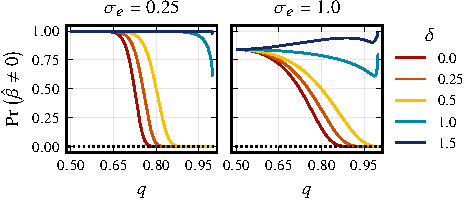
\includegraphics[]{plots/selection_probability.pdf}
  \caption{%
    Probability of selection in the elastic net problem given a measurement noise level \(\sigma_\varepsilon\), a regularization parameter \(\lambda_1\), and a class balance \(q\). The scaling factor is parameterized by \(s_j = (q - q^2)^\delta\), \(\delta \geq 0\). The dotted line represents the asymptotic limit for the standardization case, \(\delta = 1/2\). }
  \label{fig:selection-probability}
\end{figure}

In \Cref{thm:classbalance-bias}, we show what the
bias is under mean-centering and scaling with \(s_j = (q - q^2)^\delta\), \(\delta \geq 0\).

\begin{theorem}
  \label{thm:classbalance-bias}
  If \(\vec{x}_j\) is a binary feature with class balance \(q \in (0, 1)\), \(\lambda_1 \in (0,\infty)\), \(\lambda_2 \in [0,\infty)\), \(\sigma_\varepsilon > 0\), and \(s_j = (q - q^2)^{\delta}\), \(\delta \geq 0\)  then
  \[
    \lim_{q \rightarrow 1^+} \E \hat{\beta}_j =
    \begin{cases}
      0                                                                                                  & \text{if } 0 \leq \delta < \frac{1}{2}, \\
      \frac{2n \beta_j^*}{n + \lambda_2} \cdf\left(-\frac{\lambda_1}{\sigma_\varepsilon \sqrt{n}}\right) & \text{if } \delta = \frac{1}{2},        \\
      \beta^*_j                                                                                          & \text{if } \delta \geq 1.
    \end{cases}
  \]
\end{theorem}

\begin{corollary}[Bias in Ridge Regression]
  \label{cor:ridge-bias}
  Asume the conditions of \Cref{thm:classbalance-bias} but that \(\lambda_1 = 0\). Then
  \[
    \lim_{q \rightarrow 1^+} \E \hat{\beta}_j =
    \begin{cases}
      0                                         & \text{if } 0 \leq \delta < 1/2, \\
      \frac{\beta_j^*}{1 + \frac{\lambda_2}{n}} & \text{if } \delta = 1/2,        \\
      0                                         & \text{if } \delta > 1/2.
    \end{cases}
  \]
\end{corollary}

\Cref{thm:classbalance-bias} shows that the bias of the elastic net estimator when \(0 \leq \delta < 1/2\), which includes to the case of min--max and max--abs normalization (no scaling), approaches
\(-\beta_j^*\) as \(q \rightarrow 1^+\). When \(\delta = 1/2\) (standardization), the lasso estimate does not vanish completely. Instead, it approaches the
true coefficient scaled by the probability that a standard normal variable is smaller than \(\beta_j^*\sqrt{n}\sigma_\varepsilon^{-1}\). For \(\delta \geq 1\), the
estimate is unbiased asymptotically. The last fact may seem somewhat counterintuitive but is a consequence of the variance of the distribution of the estimator exploding as \(q \rightarrow 1^+\).

\begin{theorem}
  \label{thm:classbalance-variance}
  If \(\vec{x}_j\) is a binary feature with class balance \(q \in (0, 1)\) and \(\lambda_1,\lambda_2 \in (0,\infty)\), \(\sigma_\varepsilon > 0\), and \(s_j = (q - q^2)^{\delta}\), \(\delta \geq 0\), then
  \[
    \lim_{q \rightarrow 1^+} \var \hat{\beta}_j =
    \begin{cases}
      0      & \text{if } 0 \leq \delta < \frac{1}{2}, \\
      \infty & \text{if } \delta \geq \frac{1}{2}.
    \end{cases}
  \]
\end{theorem}

\begin{corollary}[Variance in Ridge Regression]
  \label{cor:ridge-variance}
  Assume the conditions of \Cref{thm:classbalance-variance} but that \(\lambda_1 = 0\). Then
  \[
    \lim_{q \rightarrow 1^+} \var \hat{\beta}_j =
    \begin{cases}
      0                                          & \text{if } 0 \leq \delta < 1/4, \\
      \frac{\sigma_\varepsilon^2 n}{\lambda_2^2} & \text{if } \delta = 1/4,        \\
      \infty                                     & \text{if } \delta > 1/4.
    \end{cases}
  \]
\end{corollary}

\begin{figure}[htpb]
  \centering
  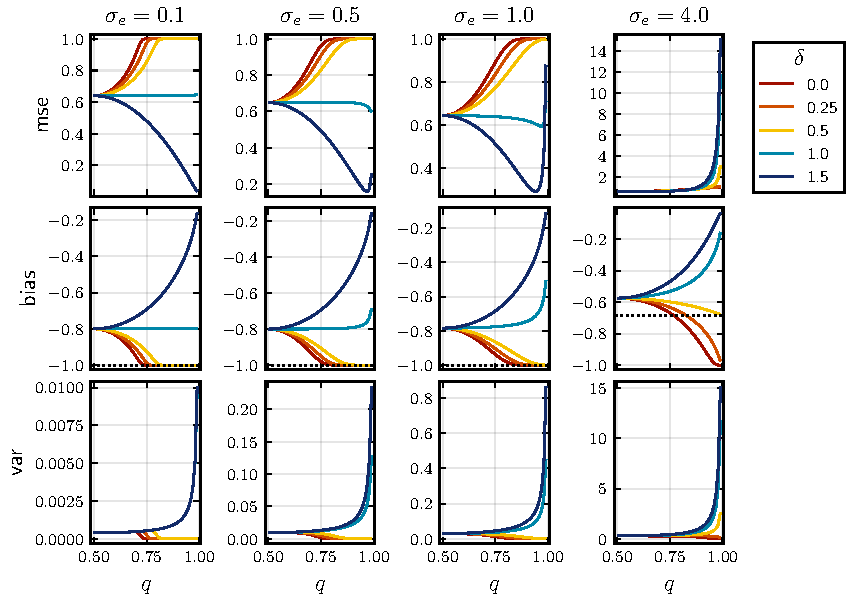
\includegraphics[]{plots/bias-var-onedim.pdf}
  \caption{%
    Bias, variance, and mean-squared error for a one-dimensional lasso problem.
    Note that \(\delta = 0\) corresponds to the case of no scaling, \(\delta = 1/2\) corresponds
    to standardization, and \(\delta = 1\) corresponds to scaling with the variance. The dotted
    lines represent the asymptotic bias of the lasso estimator in the case of \(\delta = 1/2\).
  }
  \label{fig:bias-var-onedim-lasso}
\end{figure}

\subsection{Multiple Predictors}

\begin{figure}[htpb]
  \centering
  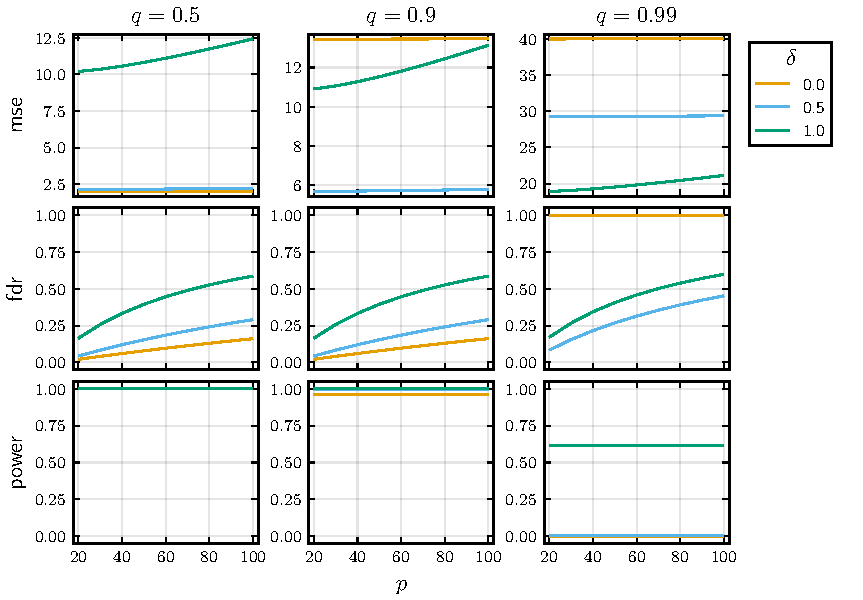
\includegraphics[]{plots/beta-bias-multidim.pdf}
  \caption{%
    Mean-squared-error, false discovery rate (FDR), and power for a lasso problem with
    \(k = 10\) true signals (nonzero \(\beta_j^*\)), varying \(p\), and \(q \in [0.5, 0.9, 0.99]\). The noise level is set at \(\sigma_\varepsilon = 1\).
  }
  \label{fig:mse-fdr-power-multidim}
\end{figure}

\section{Mixed Data}
\label{sec:mixed-data}

A natural follow-up topic to the discussion in the previous section is to consider the case where the features are of mixed type, that is, some are continuous and some are binary.
To be able to compare normalization methods with respect to these cases, we need to construct problems in which the coefficients of the continuous and binary features are, in some sense, comparable.
In this section, we will discuss what it means for a continuous and binary feature to have \emph{comparable} effects and how the choice of normalization needs to be adapted to ensure that our penalized estimates respect this notion of comparability.

In this pape, we will focus on normally distrubted continuous features. We acknowledge that this is a limiting choice, but leave it to future papers to approach this issue for other types of distributions.

We will assume that the effect of a change in the binary variable (going from 0 to 1) corresponds to a difference of two standard deviations in the normally distributed variable. We base this choice on the reasoning by \textcite{gelman2008}. In other words, if the regression coefficient of the binary variable is \(\beta^*_1\), then the effect corresponding to a normally distributed random variable is equivalent if \(\beta^*_2 = (2\sigma)^{-1} \beta_1^*\).

\begin{example}
  If \(\vec{x}_2\) is sampled from \(\normal(\mu, 2)\), then the effects of \(\vec{x}_1\) and \(\vec{x}_2\) are equivalent if \(\beta_1^* = 1\) and \(\beta_2^* = 0.25\).
\end{example}

Our particular choice of two standard deviations is not critical for our results, which hold for any other choice, as long it is linear with respect to the standard deviation of the normally distributed variable.

On the other hand, we also assume that the effects are equivalent irrespective of the class balance of the binary feature. In other words, we say that two binary features \(\vec{x}_1\) and \(\vec{x}_3\) have equivalent effects as long as \(\beta_1^* = \beta_3^*\), even if the values in \(\vec{x}_1\) are spread evenly between zeros and ones and those of \(\vec{x}_3\) are all zeros except for one. We will see that this is a fundamental assumption upon which our results hinge entirely.

We will cover cases where the continuous feature is not normally distributed on a case-by-case basis as we proceed through the paper.



\section{Experiments}

In the following sections we present the results of our experiments. For all simulated data
we generate our response vector according to \(\vec{y} = \mat{X}\vec{\beta}^* +
\vec{\varepsilon},\) with \(\vec{\varepsilon} \sim \normal(\vec{0}, \sigma_\varepsilon^2
\mat{I})\). We consider two types of features: binary (quasi-Bernoulli) and quasi-normal
features. To generate binary vectors, we sample \(\ceil{nq_j}\) indexes uniformly at random
without replacement from \([n]\) and set the corresponding elements to one and the
remaining ones to zero. To generate quasi-normal features, we generate a linear sequence
\(\vec{w}\) with \(n\) values from \(10^{-4}\) to \(1 - 10^{-4}\), set \(x_{ij} =
\cdf^{-1}(w_i)\), and then shuffle the elements of \(\vec{x}_j\) uniformly at random.

We use a coordinate descent solver to optimize our models, which we have based on the
algorithm outlined by \citet{friedman2010}. All experiments were coded using the Julia
programming language~\citep{bezanson2017} and the code is available at
\url{https://github.com/jolars/normreg}.
% in the supplementary material. 
All simulated experiments were run for at least 100 iterations and, unless stated
otherwise, are presented as means $\pm$ one standard deviation (using bars or ribbons).

\subsection{Normalization in the Lasso and Ridge Regression}%
\label{sec:experiments-lassoridge}

In this section we consider fitting the lasso and ridge regression to normalized data sets.
To normalize the data, we use standardize all quasi-normal features. For binary features,
we center by mean and scale by \(s_j \propto (q_j-q_j^2)^\delta\).
% where \(\delta = 0\)
% corresponds to no scaling, \(\delta = 1/2\) to standardization, and \(\delta = 1\) to
% variance scaling.

\subsubsection{Variability and Bias in Estimates}

In our first experiment, we consider fitting the lasso to a simulated data set with
\(n=500\) observations and \(p = \num{1000}\) features, out of which the first 20 features
correspond to signals, with \(\beta_j^*\) decreasing linearly from 1 to 0.1. We introduce
dependence between the features by copying the first \(\ceil{\rho n/2}\) values from the
first feature to each of the following features. In addition, we set the class balance of
the first 20 features so that it decreases linearly on a log-scale from 0.5 to 0.99. We
estimate the regression coefficients using the lasso, setting \(\lambda_1 = 2
\sigma_\varepsilon \sqrt{2 \log p }\).

The results~(\Cref{fig:binary-decreasing}, and \Cref{fig:binary-decreasing-full} in
\Cref{sec:additional-results-biasvar}) show that class balance has considerable effect,
particularly in the case of no scaling (\(\delta = 0\)), which corroborates our theory from
\Cref{sec:theory-binary-features}. At \(q_j=0.99\), for instance, the estimate
(\(\hat{\beta}_{20}\)) is consistently zero when \(\delta = 0\). For \(\delta=1\), we see
that class imbalance increases the variance of the estimates. What is also clear is that
the variance of the estimates increase with class imbalance and that this effect increases
together with \(\delta\).

\begin{figure}[htpb]
  \centering
  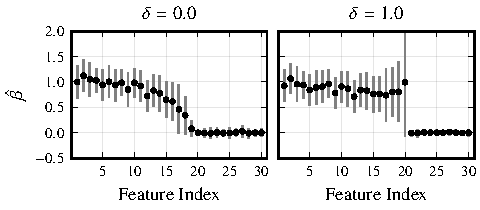
\includegraphics[]{binary_decreasing_small.pdf}
  \caption{%
    Regression coefficients for a lasso problem with binary data where \(n = 500\) and
    \(p = \num{1000}\) with 20 true signals. Here we show only the first 30
    coefficients. See \Cref{sec:experiments-lassoridge} for more information
    on the setup of this experiment.
  }
  \label{fig:binary-decreasing}
\end{figure}

\subsubsection{Predictive Performance}

In this section we examine the influence of normalization on predictive performance for
three different data sets: \data{a1a}~\citep{becker1996}, \data{rhee2006}~\citep{rhee2006},
and \data{w1a}~\citep{platt1998}.\footnote{See \Cref{sec:data-summary} for details about
  these data sets.} We evaluate performance in terms of normalized mean-squared error~(NMSE)
for lasso and ridge regression across a two-dimensional grid of \(\delta\) and \(\lambda\),
where for \(\delta\) we use a linear sequence from 0 to 1, and for \(\lambda\) a geometric
sequence from \(\lambda_\text{max}\) (the value of \(\lambda\) at which the first feature
enters the model) to \(10^{-2}\lambda_\text{max}\). We split the data into equal training
and validation set splits and for each combination of \(\lambda\) and \(\delta\) fit the
lasso or ridge to the training set.

We present the results for ridge regression in \Cref{fig:hyperopt-contours}, which shows
contour plots of the validation set error. We see that optimal setting of \(\delta\)
differs between the different data sets, suggesting that it is useful to choose \(\delta\)
by hyperparameter optimization. See
\Cref{fig:hyperopt-contours-full}~(\Cref{sec:predictive-performance-simulated}) for a plot
that includes the lasso as well.

% For
% \data{a1a}, the lasso is generally quite insensitive to the type of normalization, even if
% the optimal value is around 0.2. For ridge regression, lower values of \(\delta\) clearly
% work better. With the \data{w1a} data set, however, the relationship is flipped in the case
% of ridge regression and the optimal value is approximately 0.8. In the case of the lasso
% (for \(\data{w1a}\)), a value around 0.5 is optimal and low values (little scaling) yield
% worse prediction errors. Finally, for \data{rhee2006}, the lasso is again insensitive to
% normalization type. This is not the case for ridge, however, where a value around 0.2 is
% optimal and high values of \(\delta\) yield worse prediction errors.

\begin{figure}[htpb]
  \centering
  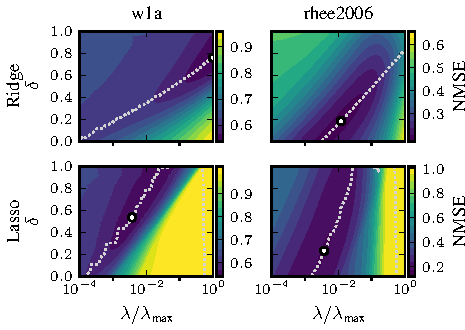
\includegraphics[]{hyperopt_surfaces_small.pdf}
  \caption{%
    Contour plots of normalized validation set mean-squared error (NMSE)
    for \(\delta\) and \(\lambda\) in ridge regression on
    three real data sets. The
    dotted path shows the smallest NMSE as a function of \(\lambda\) and the circles mark
    combinations with the lowest error.
  }
  \label{fig:hyperopt-contours}
\end{figure}

% We would like to point out that there is a dependency between \(\lambda\) and \(\delta\)
% that make it difficult to interpret the relationship between them and the error. This comes
% from the fact that scaling with a smaller value (as in \(\delta = 1\)) increases the sizes
% of the vectors, which means that the level of penalization is relaxed, relatively speaking.

In \Cref{sec:predictive-performance-simulated}, we extend these results with experiments on
simulated data under various class balances and signal-to-noise ratios, again showing that
normalization has an impact on predictive preformance.

\subsubsection{Mixed Data}\label{sec:experiments-mixed-data}

In \Cref{sec:mixed-data} we showed theoretically that care needs to be taken when
normalizing mixed data. Here we verify the theory through simulations. We construct a
quasi-normal feature with mean zero and standard deviation 1/2 and a binary feature with
varying class balance \(q_j\). We set the signal-to-noise ratio to 0.5 and use \(n =
\num{1000}\). These features are constructed so that their effects are comparable under the
notion of comparability that we introduced in \Cref{sec:mixed-data} using \(\kappa = 2\).
In order to preserve the comparability for the baseline case when we have perfect class
balance, we scale by \(s_j = 2 \times (1/4)^{1-\delta}(q_j-q_j^2)^\delta\). Finally, we set
\(\lambda\) to \(\lambda_\text{max}/2\) and \(2\lambda_\text{max}\) for lasso and ridge
regression respectively.

The results~(\Cref{fig:lasso-ridge-comparison}) reflect our theoretical results from
\Cref{sec:theory}. In the case of the lasso, we need \(\delta =1\) (variance scaling) to
avoid the effect of class imbalance, whereas for ridge we instead need \(\delta =1/2\)
(standardization). As our theory suggests, this extra scaling mitigates this class-balance
dependency at the cost of added variance.
% Note that we do not see the bias reduction that
% we observed in our theoretical results for high \(q_j\) values and \(\delta \geq 1/2\) in
% \Cref{fig:lasso-ridge-comparison}. This is related to the error term (signal-to-noise
% ratio) and level of \(q_j\). We would need stronger class imbalance and larger error for
% the effect to show up here.

\begin{figure}[htpb]
  \centering
  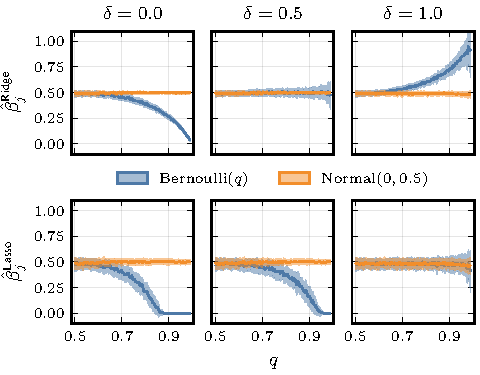
\includegraphics{mixed_data.pdf}
  \caption{%
    Lasso and ridge estimates for a two-dimensional problem where one feature is a binary
    feature with class balance \(q_j\) (\(\bernoulli(q_j)\)) and the other is quasi-normal
    with standard deviation 1/2, (\(\normal(0, 0.5)\)).
  }
  \label{fig:lasso-ridge-comparison}
\end{figure}

\subsubsection{Interactions}\label{sec:experiments-interactions}

Next, we study the effects of normalization and class balance on interactions in the lasso.
Our example consists of a two-feature problem with an added interaction term given by
\(x_{i3} = x_{i1}x_{i2}\). The first feature is binary with class balance \(q\) and the
second quasi-normal with standard deviation 0.5. We use \(n=1000\), \(\lambda_1 = n/4\),
and normalize the binary feature by mean-centering and scaling by \(\kappa (q - q^2)\),
using \(\kappa = 2\). We consider two different strategies for choosing \(s_3\): in the
first strategy, which we call \emph{Strategy 1}, we simply standardize the resulting
interaction feature.
% TODO: make a reference to where this is done
In the second strategy, \emph{Strategy 2} we center with mean and scale with \(s_1s_2\)
(the product of the scales of the binary and normal features).

The results for \(\bm{\beta}^* = \bm{1}\)~(\Cref{fig:interactions}) show that only strategy
2 estimates the effect of the interaction correctly. Strategy 1, meanwhile, only selects
the correct model if the class balance of the binary feature is close to 1/2 and in general
shrinks the coefficient too much. See
\Cref{fig:interactions-full}~(\Cref{sec:additional-experiments-interactions}) for results
on different choices of \(\bm{\beta}^*\).

\begin{figure}[htpb]
  \centering
  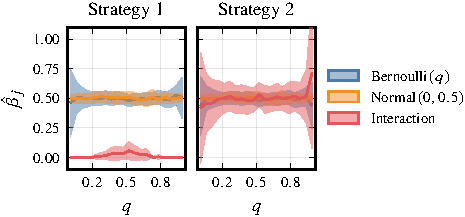
\includegraphics[]{interactions-classbalance-small.pdf}
  \caption{%
    Lasso estimates for a problem with a binary feature, a quasi-normal feature, and
    an interaction feature. We have set \(\bm{\beta}^* = \bm{1}\) and use two different normalization strategies where
    Strategy 1 represents standardization and Strategy 2 is mean-centering
    together with scaling by \(s_1 s_2\).
  }
  \label{fig:interactions}
\end{figure}

\subsection{The Weighted Elastic Net}

The weighted elastic net can be used as an alternative to normalization to correct for
class balance bias when \(\lambda_1 > 0\) and \(\lambda_2 >0\). To simplify the
presentation, we parameterize the elastic net as \(\lambda_1 = \alpha \lambda \) and
\(\lambda_2 = (1-\alpha) \lambda\), so that \(\alpha\) controls the balance between the
ridge and lasso. We conduct an experiment with the same setup as in
\Cref{sec:experiments-mixed-data}, but here we use the weighted elastic net instead with
\(\alpha = 0.5\) (See \Cref{sec:additional-experiments-weighted-elnet} for results using
other setting for \(\alpha\)). We use \(n=1000\) and vary \(\omega\), using the weights
\(u_j = v_j = (q_j - q_j^2)^{\omega}\) as we suggested in \Cref{sec:binary-weighting}. Our
results (\Cref{fig:mixed-data-elnet}) show that \(\omega = 1\) leads to seemingly unbiased
estimates.

\begin{figure}[htpb]
  \centering
  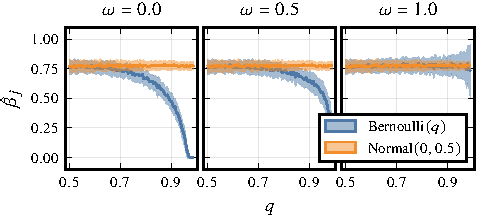
\includegraphics{mixed_data_elnet_small.pdf}
  \caption{%
    Weighted elastic net estimates for \(\alpha = 0.5\) for a problem with a binary
    feature with class balance \(q\) (\(\bernoulli(q)\)) and quasi-normal
    with standard deviation 1/2 (\(\normal(0, 0.5)\)). \(\omega\) indicates
    the scaling of the penalty weights.
  }
  \label{fig:mixed-data-elnet}
\end{figure}



% \subsubsection*{Broader Impact Statement}
%
% In this optional section, TMLR encourages authors to discuss possible repercussions of their work,
% notably any potential negative impact that a user of this research should be aware of.
% Authors should consult the TMLR Ethics Guidelines available on the TMLR website
% for guidance on how to approach this subject.

% \subsubsection*{Acknowledgments}
%
% Use unnumbered third level headings for the acknowledgments. All
% acknowledgments, including those to funding agencies, go at the end of the paper.
% Only add this information once your submission is accepted and deanonymized.

\bibliography{normreg}
\bibliographystyle{tmlr}

\appendix

\section{Appendix}

\section{Proofs}

\subsection{Proof of \Cref{thm:maxabs-gev}}

If \(X_i \sim \normal(\mu, \sigma)\), then \(|X_i| \sim \fnormal(\mu,\sigma)\). By the Fisher--Tippett--Gnedenko theorem, we know that \((\max_i |X_i| - b_n) / a_n\) converges in distribution to either the Gumbel, Fréchet, or Weibull distribution, given a proper choice of \(a_n > 0\) and \(b_n \in \mathbb{R}\). A sufficient condition for convergence to the Gumbel distribution for a absolutely continuous cumulative distribution function~\citep[Theorem 10.5.2]{nagaraja2003} is
\[
  \lim_{x \rightarrow \infty} \frac{d}{dx}\left(\frac{1- F(x)}{f(x)}\right) = 0.
\]
We have
\[
  \begin{aligned}
    \frac{1 - F_Y(x)}{f_Y(x)} & = \frac{1 - \frac{1}{2}\erf{\left(\frac{x - \mu}{\sqrt{2\sigma^2}}\right)} - \frac{1}{2}\erf{\left(\frac{x + \mu}{\sqrt{2\sigma^2}}\right)}}{\frac{1}{\sqrt{2\pi\sigma^2}}e^{\frac{-(x-\mu)^2}{2\sigma^2}} + \frac{1}{\sqrt{2\pi\sigma^2}}e^{\frac{-(x+\mu)^2}{2\sigma^2}}} \\
                              & = \frac{2 - \cdf\left(\frac{x - \mu}{\sigma}\right) - \cdf\left(\frac{x + \mu}{\sigma}\right)}{\frac{1}{\sigma}\left(\pdf\left(\frac{x - \mu}{\sigma}\right) + \pdf\left(\frac{x + \mu}{\sigma}\right)\right)}                                                              \\
                              & \rightarrow \frac{\sigma(1 - \cdf(x))}{\pdf(x)} \text{ as } n \rightarrow n,
  \end{aligned}
\]
where \(\pdf\) and \(\cdf\) are the probability distribution and cumulative density functions of the standard normal distribution respectively.
Next, we follow \citet[example 10.5.3]{nagaraja2003} and observe that
\[
  \frac{d}{dx} \frac{\sigma(1 - \cdf(x))}{\pdf(x)} = \frac{\sigma x (1 - \cdf(x))}{\pdf(x)} - \sigma \rightarrow 0 \text{ as } x \rightarrow \infty
\]
since
\[
  \frac{1 - \cdf(x)}{\pdf(x)} \sim \frac{1}{x}.
\]
In this case, we may take \(b_n = F_Y^{-1}(1 - 1/n)\) and \(a_n = \big(n f_Y(b_n)\big)^{-1}\).

\subsection{Proof of \Cref{thm:classbalance-bias}}

Since \(s_j = (q - q^2)^\delta\), we have
\begin{align*}
  \mu    & = \beta_j^* n (q - q^2)^{1 - \delta}                     & \frac{\theta}{\sigma} & = -a \sqrt{q(1-q)} - b (q - q^2)^{\delta - 1/2},           \\
  \sigma & = \sigma_\varepsilon \sqrt{n} (q - q^2)^{1/2 - \delta},  & \frac{\gamma}{\sigma} & = a \sqrt{q(1-q)} - b (q - q^2)^{\delta - 1/2},            \\
  d_j    & = n (q - q^2)^{1 - \delta} + \lambda_2 (q - q^2)^\delta, & \frac{\theta}{d_j}    & = -\beta_j^* - \frac{\lambda_1 (q - q^2)^{\delta - 1}}{n}, \\
  \theta & = -\beta^*_j n (q - q^2)^{1-\delta} - \lambda_1,         & \frac{\gamma}{d_j}    & = \beta_j^* - \frac{\lambda_1 (q - q^2)^{\delta - 1}}{n},  \\
  \gamma & = \beta^*_j n (q - q^2)^{1-\delta} - \lambda_1,
\end{align*}
with
\[
  a = \frac{\beta_j^* \sqrt{n}}{\sigma_\varepsilon} \qquad \text{and} \qquad b = \frac{\lambda_1}{\sigma_\varepsilon \sqrt{n}}.
\]

We are interested in
\begin{equation}
  \label{eq:eval-qlimit}
  \lim_{q \rightarrow 1^+} \E \hat{\beta}_j =\lim_{q \rightarrow 1^+}\frac{1}{d}\left(-\theta \cdf\left(\frac{\theta}{\sigma}\right) - \sigma \pdf\left(\frac{\theta}{\sigma}\right) + \gamma \cdf\left(\frac{\gamma}{\sigma}\right) + \sigma \pdf\left(\frac{\gamma}{\sigma}\right)\right).
\end{equation}
Before we proceed, note the following limits, which we will make repeated use of throughout the proof.
\begin{equation}
  \label{eq:eval-sigma-limits}
  \lim_{q \rightarrow 1^+} \frac{\theta}{\sigma} = \lim_{q \rightarrow 1^+} \frac{\gamma}{\sigma} =
  \begin{cases}
    -\infty & \text{if } 0 \leq \delta < \frac{1}{2}, \\
    -b      & \text{if } \delta = \frac{1}{2},        \\
    0       & \text{if } \delta > \frac{1}{2},
  \end{cases}
\end{equation}

Starting with the terms involving \(\cdf\) inside the limit in \Cref{eq:eval-qlimit}, for now assuming that they are well-defined and that the limits of the remaining terms also exist seperately, we have
\begin{align}
   & \lim_{q \rightarrow 1^+} \left(-\frac{\theta}{d} \cdf\left(\frac{\theta}{\sigma}\right) + \frac{\gamma}{d_j} \cdf \left(\frac{\gamma}{\sigma}\right)\right)                                                                                                                                                                                      \nonumber                                                        \\
   & = \lim_{q \rightarrow 1^+} \Bigg(\left(\frac{\beta_j^* n}{n + \lambda_2 (q-q^2)^{2\delta - 1}} + \frac{\lambda_1}{n(q-q^2)^{1-\delta} + \lambda_2 (q-q^2)^{\delta}} \right) \cdf \left(\frac{\theta}{\sigma}\right)  \nonumber                                                                                                                                                                                    \\
   & \phantom{= \lim_{q \rightarrow 1^+} \Bigg( } + \left(\frac{\beta_j^* n}{n + \lambda_2 (q-q^2)^{2\delta - 1}} - \frac{\lambda_1}{n(q-q^2)^{1-\delta} + \lambda_2 (q-q^2)^{\delta}} \right)\cdf \left(\frac{\gamma}{\sigma}\right) \Bigg) \nonumber                                                                                                                                                                 \\
   & = \lim_{q \rightarrow 1^+} \frac{\beta_j^*n}{n + \lambda_2 (q-q^2)^{2\delta - 1}}\left(\cdf \left(\frac{\theta}{\sigma}\right) + \cdf \left(\frac{\gamma}{\sigma}\right) \right)                                                                                                                                                                                                                        \nonumber \\
   & \phantom{={}} +  \lim_{q \rightarrow 1^+}\frac{\lambda_1}{n(q-q^2)^{1-\delta} + \lambda_2(q -q^2)^{\delta}} \left(\cdf \left(\frac{\theta}{\sigma}\right) - \cdf \left(\frac{\gamma}{\sigma}\right)\right). \label{eq:eval-qlimit-terms}
\end{align}
Considering the first term in \Cref{eq:eval-qlimit-terms}, we see that
\[
  \lim_{q \rightarrow 1^+} \frac{\beta_j^*n}{n + \lambda_2 (q-q^2)^{2\delta - 1}}\left(\cdf \left(\frac{\theta}{\sigma}\right) + \cdf \left(\frac{\gamma}{\sigma}\right) \right)  =
  \begin{cases}
    0                                            & \text{if } 0 \leq \delta < 1/2, \\
    \frac{2n \beta_j^*}{n + \lambda_2} \cdf (-b) & \text{if } \delta = 1/2,        \\
    \beta_j^*                                    & \text{if } \delta > 1/2.
  \end{cases}
\]
For the second term in \Cref{eq:eval-qlimit-terms}, we start by observing that if
\(\delta = 1\), then \(q(1-q)^{\delta - 1} = 1\), and if \(\delta > 1\), then \(\lim_{q\rightarrow 1^+}(q - q^2)^{\delta - 1} = 0\). Moreover, the arguments of \(\cdf\) approach 0 in the limit for \(\delta \geq 1\), which means that the entire term vanishes in both cases (\(\delta \geq 1\)).

For \(0 \leq \delta < 1\), the limit is indeterminite of the form \(\infty \times 0\). We define
\[
  f(q) = \cdf \left(\frac{\theta}{\sigma}\right) - \cdf \left(\frac{\gamma}{\sigma}\right)
  \qquad\text{and}\qquad
  g(q) = n(q - q^2)^{1-\delta} + \lambda_2(q - q^2)^\delta,
\]
such that we can express the limit as \(\lim_{q \rightarrow 1^+}f(q)/g(q)\). The corresponding derivatives are
\[
  \begin{aligned}
    f'(q) & = \left(-\frac{a}{2}(1-2q)(q - q^2)^{-1/2} - b(\delta - 1/2)(1-2q)(q - q^2)^{\delta - 3/2}\right)\pdf\left(\frac{\theta}{\sigma}\right)                 \\
          & \phantom{= {}} - \left(-\frac{a}{2}(1-2q)(q - q^2)^{-1/2} - b(\delta - 1/2)(1-2q)(q - q^2)^{\delta - 3/2}\right)\pdf\left(\frac{\gamma}{\sigma}\right), \\
    g'(q) & = n(1 - \delta)(1-2q)(q - q^2)^{-\delta} + \lambda_2 \delta(1 - 2q) (q - q^2)^{\delta - 1}
  \end{aligned}
\]
Note that \(f(q)\) and \(g(q)\) are both differentiable and \(g'(q) \neq 0\) everywhere in the interval \((1/2, 1)\). Now note that we have
\begin{multline}
  \label{eq:eval-qlimit-secondterm}
  \frac{f'(q)}{g'(q)} = \frac{1}{n(1-\delta)(q-q^2)^{1/2-\delta} + \lambda_2 \delta (1-2q)(q - q^2)^{\delta-1/2}} \\
  \times \left(\left(-\frac{a}{2} - b(\delta - 1/2)(q - q^2)^{\delta - 1}\right)\pdf\left(\frac{\theta}{\sigma}\right) - \left(\frac{a}{2} - b(\delta - 1/2)(q - q^2)^{\delta - 1}\right)\pdf\left(\frac{\gamma}{\sigma}\right) \right).
\end{multline}
For \(0 \leq \delta < 1/2\), $\lim_{q \rightarrow 1^+}f'(q)/g'(q) = 0$ since the exponential terms of \(\pdf\) in \Cref{eq:eval-qlimit-secondterm} dominate in the limit.

For \(\delta = 1/2\), we have
\[
  \lim_{q \rightarrow 1^+} \frac{f'(q)}{g'(q)} = -\frac{a}{n + \lambda_2} \lim_{q \rightarrow 1^+}\left(\pdf\left(\frac{\theta}{\sigma}\right) + \pdf\left(\frac{\gamma}{\sigma}\right)\right) = -\frac{a}{n + \lambda_2} \pdf(-b)
\]
so that we can use L'Hôpital's rule to show that the second term in \Cref{eq:eval-qlimit-terms} becomes
\begin{equation}
  \label{eq:eval-qlimit-stdcase}
  -\frac{2\beta_j^*\lambda_1\sqrt{n}}{\sigma_\varepsilon(n + \lambda_2)} \pdf\left(\frac{-\lambda_1}{\sigma_\varepsilon\sqrt{n}}\right).
\end{equation}

For \(\delta > 1/2\), we have
\[
  \begin{aligned}
    \lim_{q \rightarrow 1^+} \frac{f'(q)}{g'(q)} & = \lim_{q \rightarrow 1^+} \frac{-\frac{a}{2}\left(\pdf\left(\frac{\theta}{\sigma}\right) + \pdf\left(\frac{\gamma}{\sigma}\right)\right)}{n(1-\delta)(q - q^2)^{1/2 - \delta} + \lambda_2 \delta(1 - 2q)(q - q^2)^{\delta - 1/2}}                                                       \\
                                                 & \phantom{= {}} + \lim_{q \rightarrow 1^+} \frac{b(\delta - 1/2)\left(\pdf\left(\frac{\gamma}{\sigma}\right) - \pdf\left(\frac{\theta}{\sigma}\right)\right)}{n(1 - \delta)(q - q^2)^{3/2 - 2\delta} + \lambda_2 \delta (1 - 2q)(q - q^2)^{1/2}}                                          \\
                                                 & = 0 + \lim_{q \rightarrow 1^+} \frac{b(\delta - 1/2) e^{-\frac{1}{2}\left(a^2(q - q^2) + b^2(q - q^2)^{2\delta - 1}\right)}\left(e^{-ab(q-q^2)^\delta} - e^{ab(q-q^2)^\delta}\right)}{\sqrt{2\pi}\left(n(1-\delta)(q - q^2)^{3/2 - 2\delta} + \lambda_2\delta(1-2q)(q-q^2)^{1/2}\right)} \\
                                                 & = 0
  \end{aligned}
\]
since the exponential term in the numerator dominates.

Now we proceed to consider the terms involving \(\pdf\) in \Cref{eq:eval-qlimit}. We have
\begin{equation}
  \label{eq:eval-qlimit-pdfterm}
  \lim_{q \rightarrow 1^+} \frac{\sigma}{d} \left(\pdf \left(\frac{\gamma}{\sigma}\right) - \pdf \left(\frac{\theta}{\sigma}\right)\right)
  = \sigma_\varepsilon \sqrt{n} \lim_{q \rightarrow 1^+} \frac{ \pdf\left(\frac{\gamma}{\sigma}\right) - \pdf\left(\frac{\theta}{\sigma}\right)}{n(q-q^2)^{1/2} + \lambda_2(q - q^2)^{2\delta - 1/2}}
\end{equation}
For \(0 \leq \delta < 1/2\), we observe that the exponential terms in \(\pdf\) dominate in the limit, and so we can distribute the limit and consider the limits of the respective terms individually, which both vanish.

For \(\delta \geq 1/2\), the limit in \Cref{eq:eval-qlimit-pdfterm} has an indeterminate form of the type \(\infty \times 0\). Define
\[
  u(q) = \pdf\left(\frac{\gamma}{\sigma}\right) - \pdf\left(\frac{\theta}{\sigma}\right)
  \qquad\text{and}\qquad
  v(q) = n(q - q^2)^{1/2} + \lambda_2 (q - q^2)^{2\delta - 1/2}
\]
which are both differentiable in the interval \((1/2, 1)\) and \(v'(q) \neq 0\) everywhere in this interval. The derivatives are
\[
  \begin{aligned}
    u'(q) & = -\pdf\left(\frac{\gamma}{\sigma}\right)\frac{\gamma}{\sigma} \left(\frac{1}{2}\left(a(1-2q)(q - q^2)^{-1/2}\right) - b(\delta - 1/2)(1- 2q)(q - q^2)^{\delta - 3/2}\right)                  \\
          & \phantom{= {}} + \pdf\left(\frac{\theta}{\sigma}\right) \frac{\theta}{\sigma} \left(-\frac{1}{2}\left(a(1-2q)(q - q^2)^{-1/2}\right) - b(\delta - 1/2)(1- 2q)(q - q^2)^{\delta - 3/2}\right), \\
    v'(q) & = \frac{n}{2} (1 - 2q)(q - q^2)^{-1/2} + \lambda_2(2\delta - 1/2)(1 - 2q)(q - q^2)^{2\delta - 3/2}.
  \end{aligned}
\]
And so
\begin{equation}
  \begin{split}
    \frac{u'(q)}{v'(q)} = \frac{1}{n + \lambda_2(4\delta - 1)(q - q^2)^{2\delta - 1}}  \Bigg( & -\left(a - b(2\delta - 1)(q - q^2)^{\delta - 1}\right) \pdf\left(\frac{\gamma}{\sigma}\right) \frac{\gamma}{\sigma} \\ & - \left(a + b(2\delta - 1)(q - q^2)^{\delta - 1}\right)\pdf\left(\frac{\theta}{\sigma}\right) \frac{\theta}{\sigma}\Bigg).
  \end{split}
\end{equation}
Taking the limit, rearranging, and assuming that the limits of the separate terms exist, we obtain
\begin{multline}
  \label{eq:eval-qlimit-pdfterm-split}
  \lim_{q \rightarrow 1^+} \frac{u'(q)}{v'(q)} = - a \lim_{q \rightarrow 1^+}  \frac{1}{n + \lambda_2 (4 \delta - 1)(q - q^2)^{2\delta - 1}} \left( \pdf\left(\frac{\gamma}{\sigma}\right)\frac{\gamma}{\sigma} + \pdf\left(\frac{\theta}{\sigma}\right)\frac{\theta}{\sigma}\right) \\
  + b (2\delta - 1) \lim_{q \rightarrow 1^+} \frac{1}{n + \lambda_2 (4 \delta - 1)(q - q^2)^{2\delta - 1}} \bigg( \pdf\left(\frac{\gamma}{\sigma}\right) \left(a(q -q^2)^{\delta - 1/2}- b(q - q^2)^{2\delta - 3/2} \right) \\
  - \pdf\left(\frac{\theta}{\sigma}\right) \left(-a(q - q^2)^{\delta - 1/2} - b(q - q^2)^{2\delta - 3/2}\right) \bigg).
\end{multline}
For \(\delta = 1/2\), we have
\[
  \lim_{q \rightarrow 1^+} \frac{u'(q)}{v'(q)} = -\frac{a}{n + \lambda_2}\left(-b \pdf(-b) - b \pdf(-b)\right) + 0 = 2ab \pdf(-b) = \frac{2 \beta_j^* \lambda_1}{\sigma_\varepsilon^2(n + \lambda_2)} \pdf \left(\frac{-\lambda_1}{\sigma_\varepsilon\sqrt{n}}\right).
\]
Using L'Hôpital's rule, the second term in \Cref{eq:eval-qlimit-pdfterm} must consequently be
\[
  \frac{2 \beta_j^* \lambda_1\sqrt{n}}{\sigma_\varepsilon(n + \lambda_2)} \pdf \left(\frac{-\lambda_1}{\sigma_\varepsilon\sqrt{n}}\right).
\]
which cancels with \Cref{eq:eval-qlimit-stdcase}.

For \(\delta > 1/2\), we first observe that the first term in \Cref{eq:eval-qlimit-pdfterm-split} tends to zero due to \Cref{eq:eval-sigma-limits} and
the properties of the standard normal distribution. For the second term, we note that this is essentially
of the same form as \Cref{eq:eval-qlimit-secondterm} and that the limit is therefore 0 here.

\subsection{Proof of \Cref{cor:ridge-bias}}

\begin{proof}
  If \(\lambda_1 = 0\), we have \(\E \st_{\lambda_1}(Z) = \mu\) and consequently
  \[
    \E \hat{\beta}_j = \frac{\beta_j^*}{1 + \frac{\lambda_2}{n} (q - q^2)^{2\delta - 1}}.
  \]
  Then
  \[
    \lim_{q \rightarrow 1^+} \E \hat{\beta}_j = \frac{\beta_j^*}{1 + \frac{\lambda_2}{n}\lim_{q \rightarrow 1^+} (q - q^2)^{2\delta - 1}}.
  \]
  The result follows by noting that
  \[
    \lim_{q \rightarrow 1^+} (q - q^2)^{2\delta - 1} =
    \begin{cases}
      \infty    & \text{if } 0 \leq \delta < 1/2, \\
      1         & \text{if } \delta = 1/2,        \\
      \beta_j^* & \text{if } \delta > 1/2.
    \end{cases}
  \]
\end{proof}

\subsection{Proof of \Cref{thm:classbalance-variance}}

The variance of the elastic net estimator is given by
\begin{multline}
  \label{eq:varthm-var}
  \var \hat{\beta}_j = \frac{1}{d^2}\Bigg( \frac{\sigma^2}{2}\bigg(2 + \erf\left(\frac{\theta}{\sigma \sqrt{2}}\right) - \frac{\theta}{\sigma}\sqrt{\frac{2}{\pi}} \exp\left(-\frac{\theta^2}{2\sigma^2}\right) + \erf\left(\frac{\gamma}{\sigma\sqrt{2}}\right) - \frac{\gamma}{\sigma} \sqrt{\frac{2}{\pi}} \exp\left(- \frac{\gamma^2}{2\gamma^2}\right)\bigg) \\
  + 2\theta\sigma \pdf\left(\frac{\theta}{\sigma}\right) + \theta^2 \cdf\left(\frac{\theta}{\sigma}\right) + 2\gamma \sigma \pdf\left(\frac{\gamma}{\sigma}\right) + \gamma^2 \cdf\left(\frac{\gamma}{\sigma}\right) \Bigg)
  - \left(\frac{1}{d}\E \hat{\beta}_j\right)^2.
\end{multline}
We start by noting the following identities:
\[
  \begin{aligned}
    \theta^2                  & = \left(\beta_j^* n\right)^2 (q-q^2)^{2-2\delta} + \lambda_1^2 + 2\lambda_1 \beta_j^* n(q-q^2)^{1-\delta},              \\
    d^2                       & = n^2(q -q^2)^{2 - 2\delta} + 2n\lambda_2 (q-q^2) + \lambda_2^2 (q-q^2)^{2\delta},                                      \\
    \theta \sigma             & =  -\sigma_\varepsilon\left(\beta_j^* n^{3/2}(q- q^2)^{3/2-2\delta} + \sqrt{n} \lambda_1 (q-q^2)^{1/2 - \delta}\right), \\
    \frac{\theta^2}{\sigma^2} & = a^2(q-q^2) + b^2(q-q^2)^{2\delta - 1} + 2ab (q -q^2)^\delta,                                                          \\
    \frac{\sigma}{d}          & = \frac{\sigma_\varepsilon \sqrt{n}}{n(q-q^2)^\frac{1}{2} + \lambda_2 (q-q^2)^{2\delta - 1/2}}.
  \end{aligned}
\]
Expansions involving \(\gamma\), instead of \(\theta\), have identical expansions up to sign changes of the individual terms.
Also recall the definitions provided in the proof of \Cref{thm:classbalance-bias}.

Starting with the case when \(0 \leq \delta < 1/2\), we write the limit of \Cref{eq:varthm-var} as
\begin{align*}
   & \lim_{q \rightarrow }\var \hat{\beta}_j                                                                                                                                                                                                                                                                                                                                             \\
   & = \sigma_\varepsilon^2 n  \lim_{q \rightarrow 1^+} \frac{1}{\left(n(q-q^2)^{1/2} + \lambda_2(q-q^2)^{2\delta - 1/2}\right)^2}\bigg(1 + \erf\left(\frac{\theta}{\sigma \sqrt{2}}\right) - \frac{\theta}{\sigma}\sqrt{\frac{2}{\pi}} \exp\left(-\frac{\theta^2}{2\sigma^2}\right)\bigg)                                                                                               \\
   & \phantom{= {}} + \sigma_\varepsilon^2 n  \lim_{q \rightarrow 1^+} \frac{1}{\left(n(q-q^2)^{1/2} + \lambda_2(q-q^2)^{2\delta - 1/2}\right)^2}\bigg(1 + \erf\left(\frac{\gamma}{\sigma\sqrt{2}}\right) - \frac{\gamma}{\sigma} \sqrt{\frac{2}{\pi}} \exp\left(- \frac{\gamma^2}{2\sigma^2}\right)\bigg)                                                                               \\
   & \phantom{= {}}+ \lim_{q \rightarrow 1^+} \frac{2\theta\sigma}{d^2} \pdf\left(\frac{\theta}{\sigma}\right) + \lim_{q \rightarrow 1^+} \frac{\theta^2}{d^2} \cdf\left(\frac{\theta}{\sigma}\right) + \lim_{q \rightarrow 1^+} \frac{2\gamma}{d^2} \sigma \pdf\left(\frac{\gamma}{\sigma}\right) + \lim_{q \rightarrow 1^+}\frac{\gamma^2}{d^2} \cdf\left(\frac{\gamma}{\sigma}\right) \\
   & \phantom{= {}}- \left( \lim_{q\rightarrow 1^+}\frac{1}{d}\E \hat{\beta}_j\right)^2,
\end{align*}
assuming, for now, that all limits exist. Next, let
\[
  \begin{aligned}
    f_1(q) & = 1 + \erf\left(\frac{\theta}{\sigma\sqrt{2}}\right) - \frac{\theta}{\sigma}\sqrt{\frac{2}{\pi}} \exp\left(-\frac{\theta^2}{2\sigma^2}\right) , \\
    f_2(q) & = 1 + \erf\left(\frac{\gamma}{\sigma\sqrt{2}}\right) - \frac{\gamma}{\sigma}\sqrt{\frac{2}{\pi}} \exp\left(-\frac{\gamma^2}{2\sigma^2}\right) , \\
    g(q)   & = \left(n^2(q-q^2) + 2n \lambda_2 (q-q^2)^{2\delta} + \lambda_2^2 (q-q^2)^{4\delta - 1}\right)^2.
  \end{aligned}
\]
And
\begin{align*}
  f_1'(q) & = \frac{\theta^2}{\sigma^2}\sqrt{\frac{2}{\pi}}\exp\left(-\frac{\theta^2}{2\sigma^2}\right),                                    \\
  f_2'(q) & = \frac{\gamma^2}{\sigma^2}\sqrt{\frac{2}{\pi}}\exp\left(-\frac{\gamma^2}{2\sigma^2}\right),                                    \\
  g'(q)   & = (1-2q)\left((q-q^2)^{-1} + 4n\delta \lambda_2 (q-q^2)^{2\delta - 1} + \lambda_2^2 (4 \delta - 1)(q-q^2)^{4\delta - 2}\right).
\end{align*}
\(f_1\), \(f_1\) and \(g\) are differentiable in \((1/2, 1)\) and \(g'(q) \neq 0\) everywhere in this interval. \(f_1/g\) and \(f_2/g\) are indeterminate of the form \(0/0\). And we see that
\[
  \lim_{q \rightarrow 1^+} \frac{f_1'(q)}{g'(q)} = \lim_{q \rightarrow 1^+} \frac{f_2'(q)}{g'(q)} = 0
\]
due to the dominance of the exponential terms as \(\theta/\sigma\) and \(\gamma/\sigma\) both tend to \(-\infty\). Thus \(f_1/g\) and \(f_2/g\) also tend to 0 by L'Hôpital's rule.

Similar reasoning shows that
\[
  \lim_{q \rightarrow 1^+} \frac{2\theta \sigma}{d^2} \pdf \left(\frac{\theta}{\sigma}\right) = \lim_{q \rightarrow 1^+} \frac{\theta^2}{d^2} \cdf \left(\frac{\theta}{\sigma}\right) = 0.
\]
The same result applies to the respective terms involving \(\gamma\).

And since we in \Cref{thm:classbalance-bias} showed that \(\lim_{q\rightarrow 1^+} \frac{1}{d} \E \hat{\beta}_j = 0\), the limit of \Cref{eq:varthm-var} must be 0.

For \(\delta = 1/2\), we start by establishing that
\[
  \lim_{q \rightarrow 1^+} \int_{-\infty}^{-\lambda}(z+ \lambda)^2 f_Z(z) \du z = \lim_{q \rightarrow 1^+} \left(\sigma^2 \int_{-\infty}^\frac{\theta}{\sigma} y^2 \pdf(y) \du y + 2 \theta \sigma \int_{-\infty}^\frac{\theta}{\sigma} y \pdf(y) \du y + \theta^2 \int_{-\infty}^\frac{\theta}{\sigma} \pdf(y) \du y\right)
\]
is a positive constant since \(\theta/\sigma \rightarrow -b\), \(\sigma = \sigma_\varepsilon \sqrt{n}\), \(\theta \rightarrow - \lambda\), and \(\theta\sigma \rightarrow - \sigma_\varepsilon \sqrt{n}\lambda\). An identical argument can be made in the case of
\[
  \lim_{q \rightarrow 1^+} \int_{\lambda}^{\infty}(z - \lambda)^2 f_Z(z) \du z.
\]
We then have
\[
  \lim_{q \rightarrow 1^+} \frac{1}{d^2} \int_{-\infty}^{-\lambda}(z+ \lambda)^2 f_Z(z) \du z = \frac{C^+}{\lim_{q\rightarrow 1^+} d^2} = \frac{C^+}{0} = \infty,
\]
where \(C^+\) is some positive constant.
And because \(\lim_{q\rightarrow 1^+} \frac{1}{d} \E \hat{\beta}_j = \beta_j^*\)~(\Cref{thm:classbalance-bias}), the limit of \Cref{eq:varthm-var} must be \(\infty\).

Finally, for the case when \(\delta > 1/2\), we have
\begin{multline*}
  \lim_{q \rightarrow 1^+} \frac{1}{d^2} \left(\sigma^2 \int_{-\infty}^\frac{\theta}{\sigma} y^2 \pdf(y) \du y + 2 \theta \sigma \int_{-\infty}^\frac{\theta}{\sigma} y \pdf(y) \du y + \theta^2 \int_{-\infty}^\frac{\theta}{\sigma} \pdf(y) \du y\right) \\
  \begin{aligned}
    = \lim_{q \rightarrow 1^+} \Bigg( & \frac{n \sigma^2}{ \left(n (q-q^2)^{1/2} + \lambda_2(q-q^2)^{2\delta - 1/2}\right)^2} \int_{-\infty}^\frac{\theta}{\sigma} y^2 \pdf(y) \du y                                                                                          \\
                                      & - \frac{2\sigma_\varepsilon \sqrt{n}\left(\beta_j^* n (q- q^2)^{1 - \delta} - \lambda_1\right)}{\left(n(q-q^2)^{3/4 - \delta/2} + \lambda_2(q-q^2)^{3\delta / 2 - 1/4}\right)^2} \int_{-\infty}^\frac{\theta}{\sigma} y \pdf(y) \du y \\
                                      & + \left(\frac{-\beta_j^*n(q-q^2)^{1-\delta} - \lambda_1}{n(q-q^2)^{1-\delta} + \lambda_2(q-q^2)^\delta}\right)^2 \int_{-\infty}^\frac{\theta}{\sigma} \pdf(y) \du y\Bigg).
  \end{aligned}
\end{multline*}
Inspection of the exponents involving the factor \((q - q^2)\) shows that the first term inside the limit will dominate. And since the upper limit of the integrals, \(\theta/\sigma \rightarrow  0\)  as \(q \rightarrow 1^+\), the limit must be \(\infty\).

\subsection{Proof of \Cref{cor:ridge-variance}}

We have
\begin{equation*}
  \lim_{q\rightarrow 1^+}\var \hat{\beta}_j = \lim_{q \rightarrow 1^+}\frac{\sigma^2}{d_j^2} \left(\frac{\sigma_\varepsilon \sqrt{n} (q - q^2)^{1/2 - \delta}}{n (q-q^2)^{1 - \delta} + \lambda_2 (q-q^2)^\delta}\right)^2
  = \frac{\sigma_\varepsilon^2 n}{\lambda_2^2} \lim_{q \rightarrow 1^+}(q-q^2)^{1 - 4\delta},
\end{equation*}
from which the result follows directly.


\end{document}
